%%%%%%%%%%%%%%%%% DO NOT CHANGE HERE %%%%%%%%%%%%%%%%%%%% {
\documentclass[12pt,letterpaper]{article}
\usepackage{fullpage}
\usepackage[top=2cm, bottom=4.6cm, left=2.6cm, right=2.6cm]{geometry}
\usepackage{amsmath,amsthm,amsfonts,amssymb,amscd}
\usepackage{lastpage}
\usepackage{enumerate}
\usepackage{fancyhdr}
\usepackage{mathrsfs}
\usepackage{xcolor}
\usepackage{graphicx}
\usepackage{subcaption}
\usepackage{listings}
\usepackage{hyperref}
\usepackage{tikz}
\usepackage{ragged2e}
\usepackage{booktabs,tabularx}
\newcommand\mcc[1]{\multicolumn{2}{c}{#1}}
\usetikzlibrary{positioning,shapes,arrows}
\usetikzlibrary[calc]
\medskip
\hypersetup{%
  colorlinks=true,
  linkcolor=blue,
  linkbordercolor={0 0 1}
}

\setlength{\parindent}{0.0in}
\setlength{\parskip}{0.05in}
%%%%%%%%%%%%%%%%%%%%%%%%%%%%%%%%%%%%%%%%%%%%%%%%%%%%%%%%%% }

%%%%%%%%%%%%%%%%%%%%%%%% CHANGE HERE %%%%%%%%%%%%%%%%%%%% {
\newcommand\course{CSI5138[F]: Intro: DL/RL}
\newcommand\semester{Fall 2019}
\newcommand\hwnumber{4}                 % <-- ASSIGNMENT #
\newcommand\NetIDa{Ao Zhang,0300039680}           % <-- YOUR NAME
\newcommand\NetIDb{Lingfeng Zhang,0300134245}           % <-- STUDENT ID #
%%%%%%%%%%%%%%%%%%%%%%%%%%%%%%%%%%%%%%%%%%%%%%%%%%%%%%%%%% }

%%%%%%%%%%%%%%%%% DO NOT CHANGE HERE %%%%%%%%%%%%%%%%%%%% {
\pagestyle{fancyplain}
\headheight 35pt
\lhead{\NetIDa}
\lhead{\NetIDa\\\NetIDb}                 
\chead{\textbf{\Large Assignment \hwnumber}}
\rhead{\course \\ \semester}
\lfoot{}
\cfoot{}
\rfoot{\small\thepage}
\headsep 1.6em
%%%%%%%%%%%%%%%%%%%%%%%%%%%%%%%%%%%%%%%%%%%%%%%%%%%%%%%%%% }

% Define block styles
\tikzstyle{sum} = [circle, draw, minimum size=1em]
\tikzstyle{mul} = [rectangle, draw, minimum size=1em]
\tikzstyle{var} = [text width=1em, text centered, minimum size=1em]
\tikzstyle{sig} = [diamond, draw, fill=blue!20, minimum size=1em]
\tikzstyle{sqsum} = [circle, draw, fill=blue!20, minimum size=1em]
\tikzstyle{line} = [draw, -latex']

\begin{document}

\section{Design Model}

Since the performance of different models with different hyper-parameters need to be analyzed and compared, neural network structures of different models applied in this homework must be same for every datasets(in this case,only MNIST hands-writing and CIFAR10) when comparing the performance of different models. This can help us to understand the true influence of some hyper-parameters better.

There are some notes that I have to mention, before we applied the CNN to build up models, we have tried the MLP in VAE,GAN and WGAN, it worked well in all these models in MNIST hands-writing datasets but worked bad in CIFAR10 datasets. There are two reasons to illustrate this phenomenon. MNIST hands-writing datasets(28*28*1) is too simple to train, so it works well even in MLP structure models. Another reason is that MLP structure is so simple that it can not train the more complex datasets(CIFAR10,32*32*3). 

Finally, we used deep convolutional structure to build up neural network layers. We first build up our models which can work well in CIFAR10 datasets because it is more complex and harder to train than MNIST hands-writing datasets. Therefore, our base models are built as the following sections illustrate.

\subsection{Discriminator or Encoder}

The structures of the Discriminator in GAN and WGAN or the structure of the Encoder in VAE are shown as Figure ~\ref{fig:disc}
\begin{figure}[h]
    \centering
    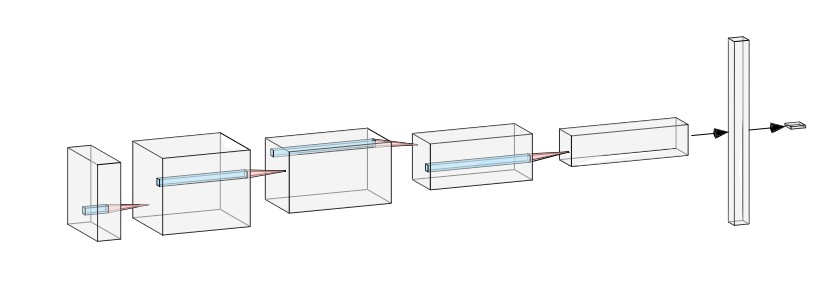
\includegraphics[width=.6\linewidth]{disc.jpg}
    \caption{\small The Structure of Discriminator or Encoder.}
    \label{fig:disc}
\end{figure}

The general description is: input images are fed into $4$ convolutional layers with stride $2$ and padding $same$, then are flatten into a big array before finally sized to the output shape by using $W \cdot X + b$.

\subsection{Generator or Decoder}

The structures of the Generators in GAN and WGAN or the structure of the Decoder in VAE are shown as Figure ~\ref{fig:gen}
\begin{figure}[h]
    \centering
    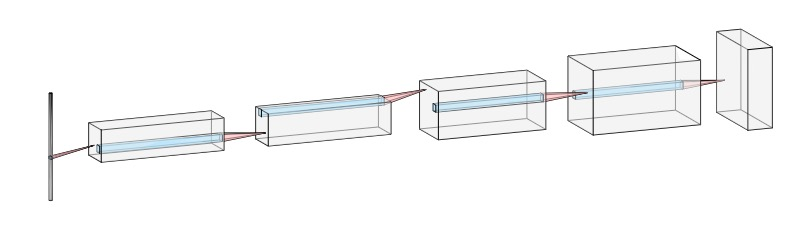
\includegraphics[width=.6\linewidth]{generator.jpg}
    \caption{\small The Structure of Generator or Decoder.}
    \label{fig:gen}
\end{figure}

The general description are: The input latent space is fed into $4$ de-convolutional layers with stride $2$ and padding $same$, with the final layer sizing it back to the same shape as the input image.

\section{MNIST Dataset}

In the following parts, we will first introduce the results and conclusions on the MNIST datasets, then we will go to the CIFAR-10 datasets in the second part.

In the following, $3$ subsections are used for describing the performance of each model as the requirements in the assignment.

In each subsection, the influence of two hyper-parameters (latent size and the number of hidden layers) will be discussed separately.

%%%%%%%%%%%%%%%%%%%%%%%%%%%%%%%%%%%%%%%%%%%%%%

\subsection{VAE}

\subsubsection{Latent Size}

First of all, let us take a look at generated images quality. The results are shown as Figure ~\ref{fig:MNIST_VAE_latent_results}

\begin{figure}[h]
    \centering
    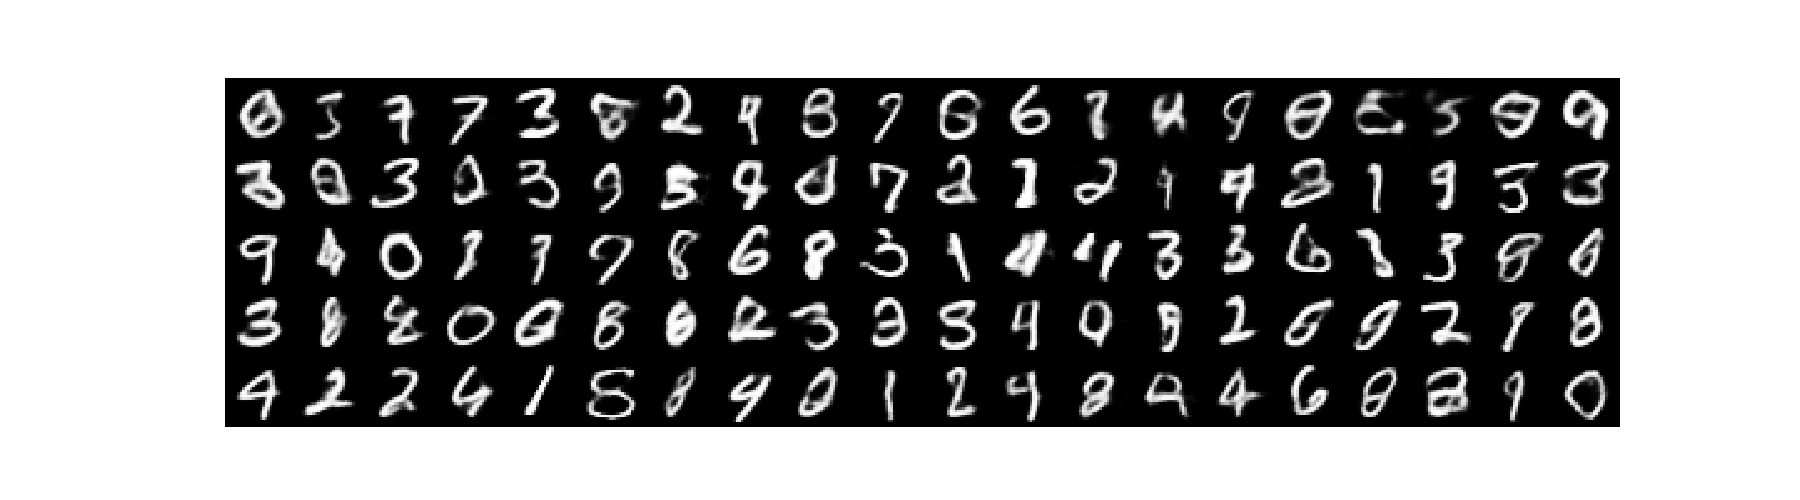
\includegraphics[width=.6\linewidth]{VAE_MNIST_0_20_256.png}
    \caption{\small A random sample with final results.}
    \label{fig:MNIST_VAE_latent_results}
\end{figure}

These images of different training time steps are shown as Figure ~\ref{fig:MNIST_VAE_latent}. In MNIST hands-writing datasets, we used 500 epochs to train. There are five rows in each images result below. For the $i$-th row, we randomly choose one epoch results in epoch range from $(i-1)*100$ to $i*100$, and we picked 20 images for each row. So the quality of images improves row by row because the model learned better and better with epoch going by. 

To compare the influence of latent size, we fixed the number of hidden layers is $3$, and then compare latent size 10,20,50,100 and 200.

\begin{figure}[h]
    \begin{subfigure}{0.49\textwidth}
    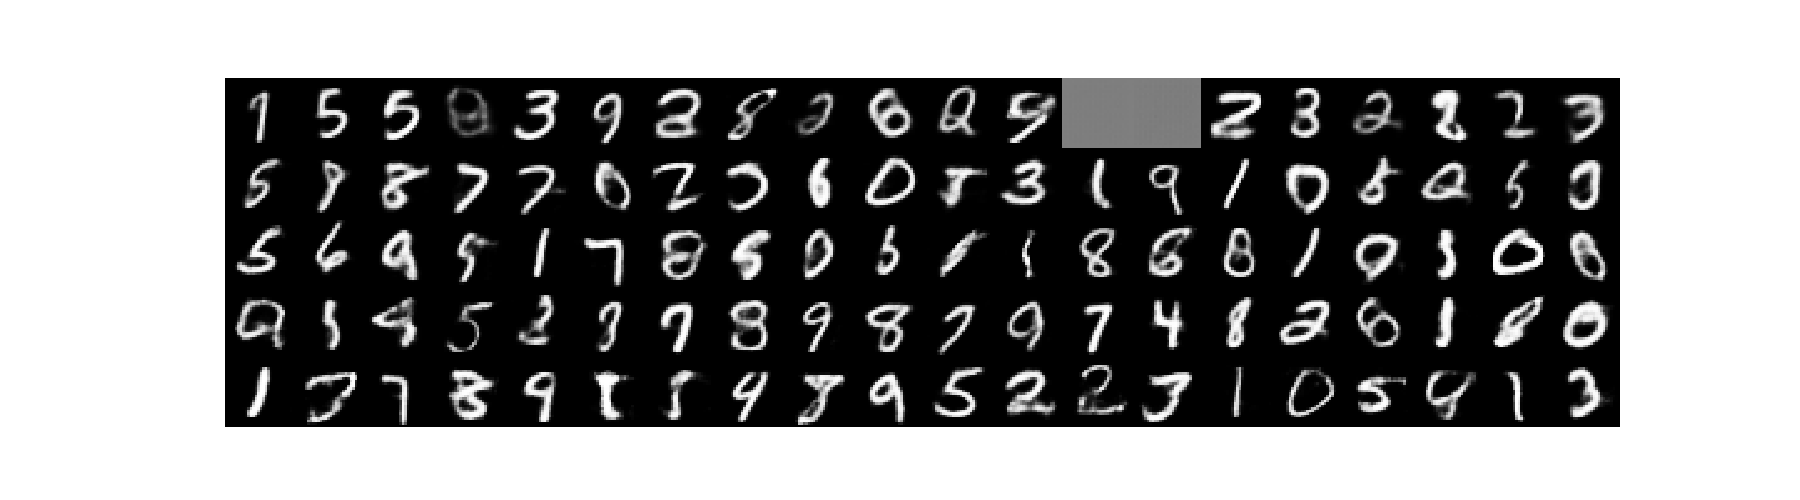
\includegraphics[width=\linewidth]{VAE_MNIST_0_10_256.png}
    \caption{\small Results on latent size 10.} \label{fig:a}
    \end{subfigure}\hspace*{\fill}
    \begin{subfigure}{0.49\textwidth}
    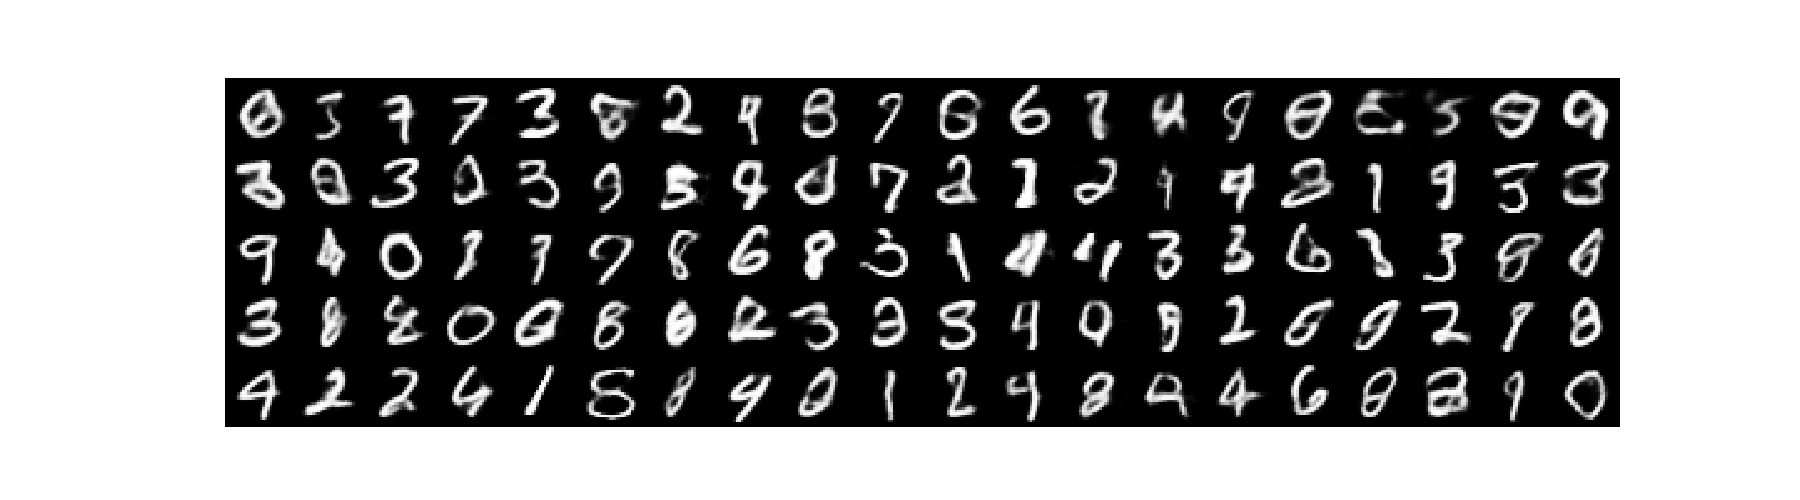
\includegraphics[width=\linewidth]{VAE_MNIST_0_20_256.png}
    \caption{\small Results on latent size 20.} \label{fig:b}
    \end{subfigure}
    
    \medskip
    \begin{subfigure}{0.49\textwidth}
    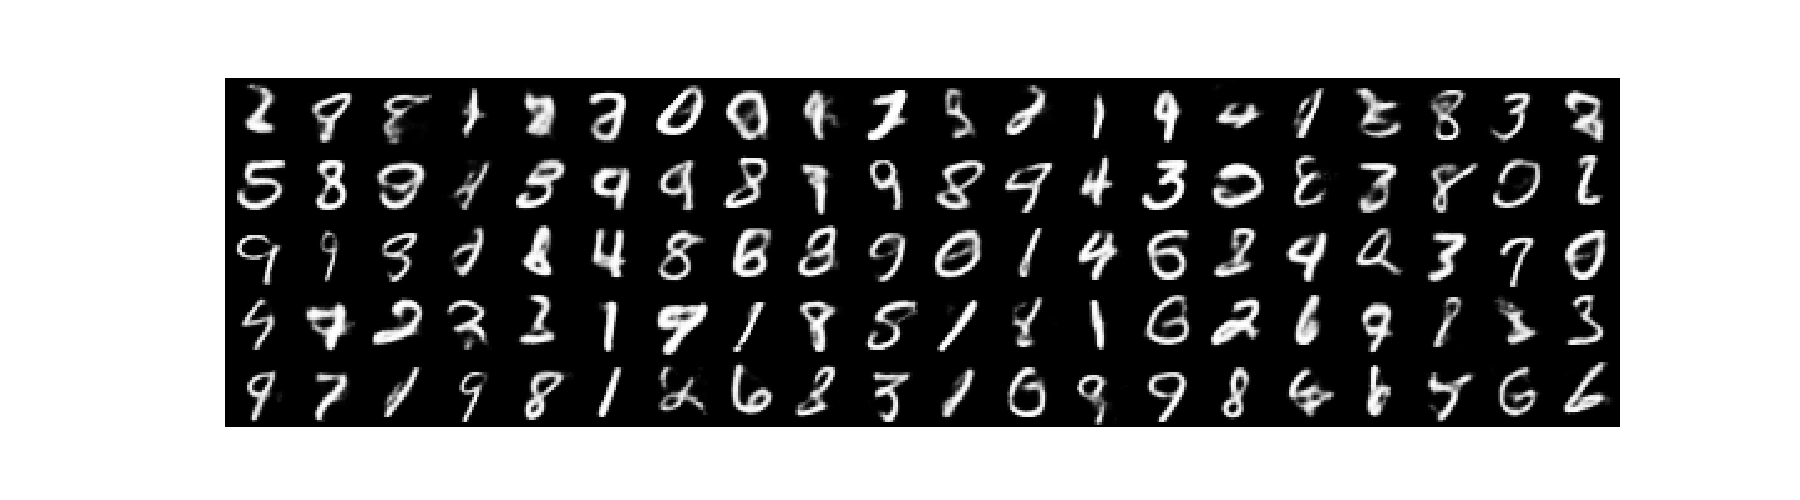
\includegraphics[width=\linewidth]{VAE_MNIST_0_50_256.png}
    \caption{\small Results on latent size 50.} \label{fig:c}
    \end{subfigure}\hspace*{\fill}
    \begin{subfigure}{0.49\textwidth}
    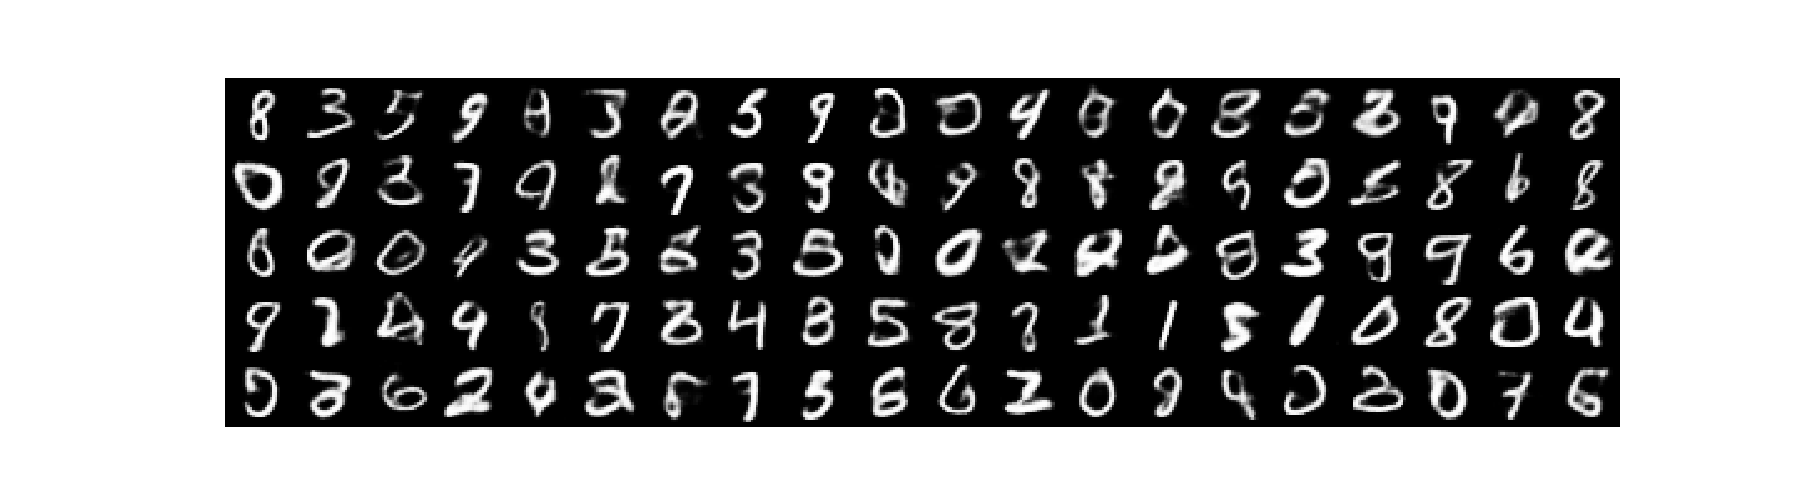
\includegraphics[width=\linewidth]{VAE_MNIST_0_100_256.png}
    \caption{\small Results on latent size 100.} \label{fig:d}
    \end{subfigure}
    
    % \medskip
    % \begin{subfigure}{0.49\textwidth}
    % 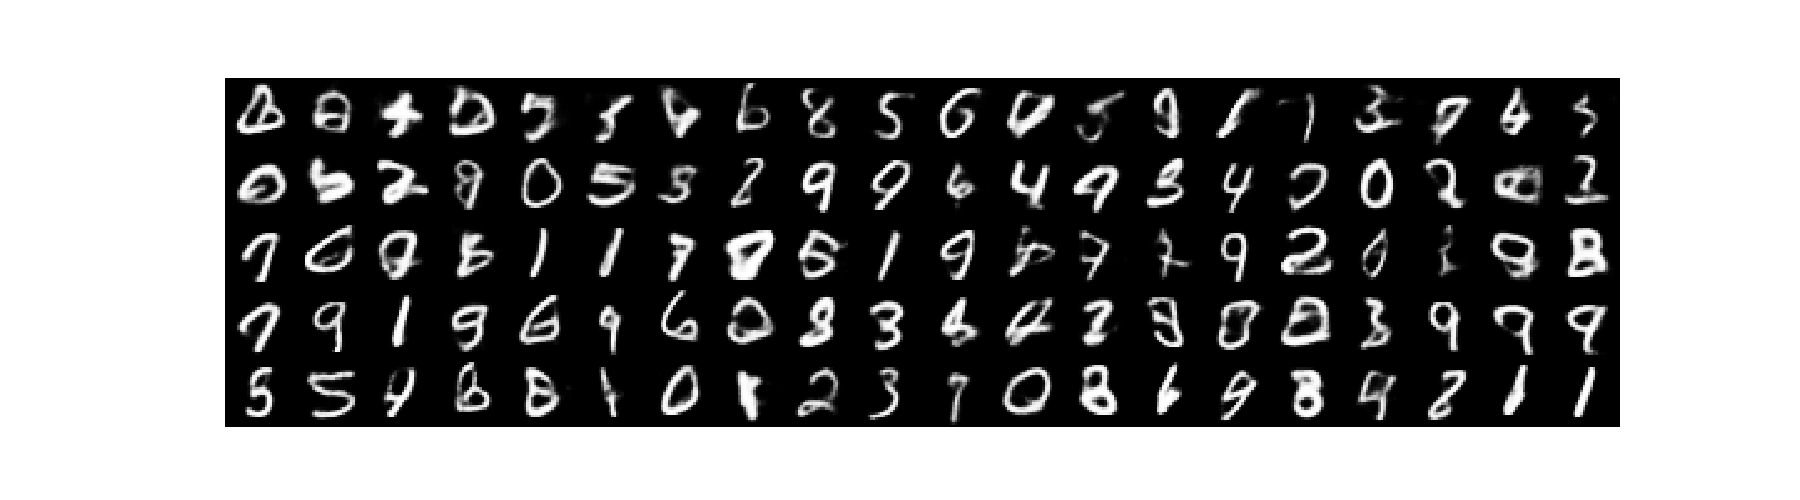
\includegraphics[width=\linewidth]{VAE_MNIST_0_200_256.png}
    % \caption{\small Results on latent size 200.} \label{fig:c}
    % \end{subfigure}
    \hspace*{\fill}
    \caption{Influence of the latent size on $5$ models, with performance increasing row by row} 
    \label{fig:MNIST_VAE_latent}
\end{figure}

As the figures show, after several thousand training steps, the model's performance becomes relatively promising.

In order to compare the training effort of the VAE model on different latent space sizes, a plot of generator loss function value is created and plotted as Figure ~\ref{fig:vae_latent}

\begin{figure}[h]
    \centering
    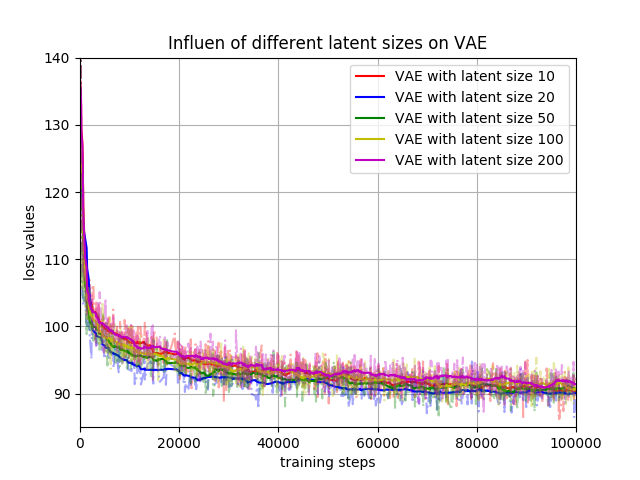
\includegraphics[width=.6\linewidth]{VAE_MNIST_latents.png}
    \caption{\small Different latent size.}
    \label{fig:vae_latent}
\end{figure}

A brief conclusion is drawn as follow,
\begin{itemize}
    \item The curves show the performances of the model on different latent size are quite similar. One may say the latent size has very slight influence on VAE. 
    \item One may spot that the performance reaches best when the latent size is $20$. This means with latent size increasing to a certain value, the performance of the model reaches an optimal value, and it will not be enhanced further with latent size keeps going up.
\end{itemize}

\subsubsection{Number of Hidden Layers}

As before, the good quality results are shown as Figure ~\ref{fig:MNIST_VAE_hidden_results}, and increasing quality results are shown as Figure ~\ref{fig:MNIST_VAE_hidden}.
\begin{figure}[h]
    \centering
    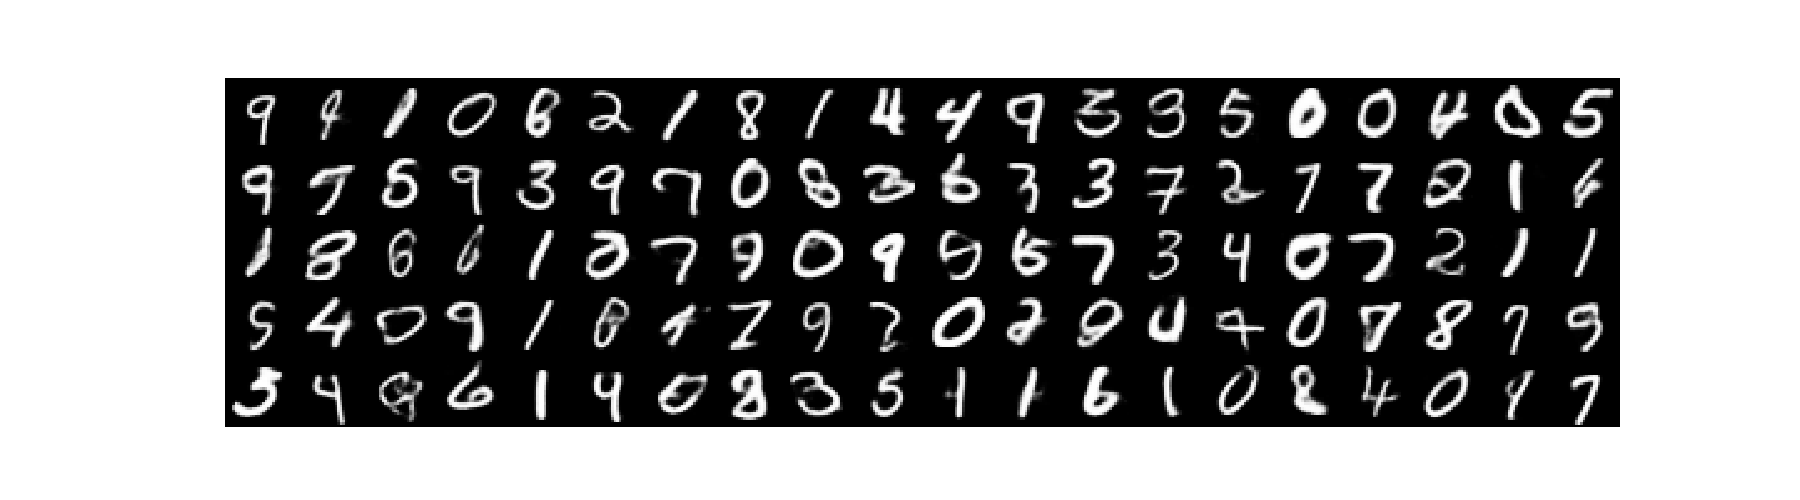
\includegraphics[width=.6\linewidth]{VAE_MNIST_2_100_256results.png}
    \caption{\small A random sample with final results.}
    \label{fig:MNIST_VAE_hidden_results}
\end{figure}

\begin{figure}[h]
    \begin{subfigure}{0.49\textwidth}
    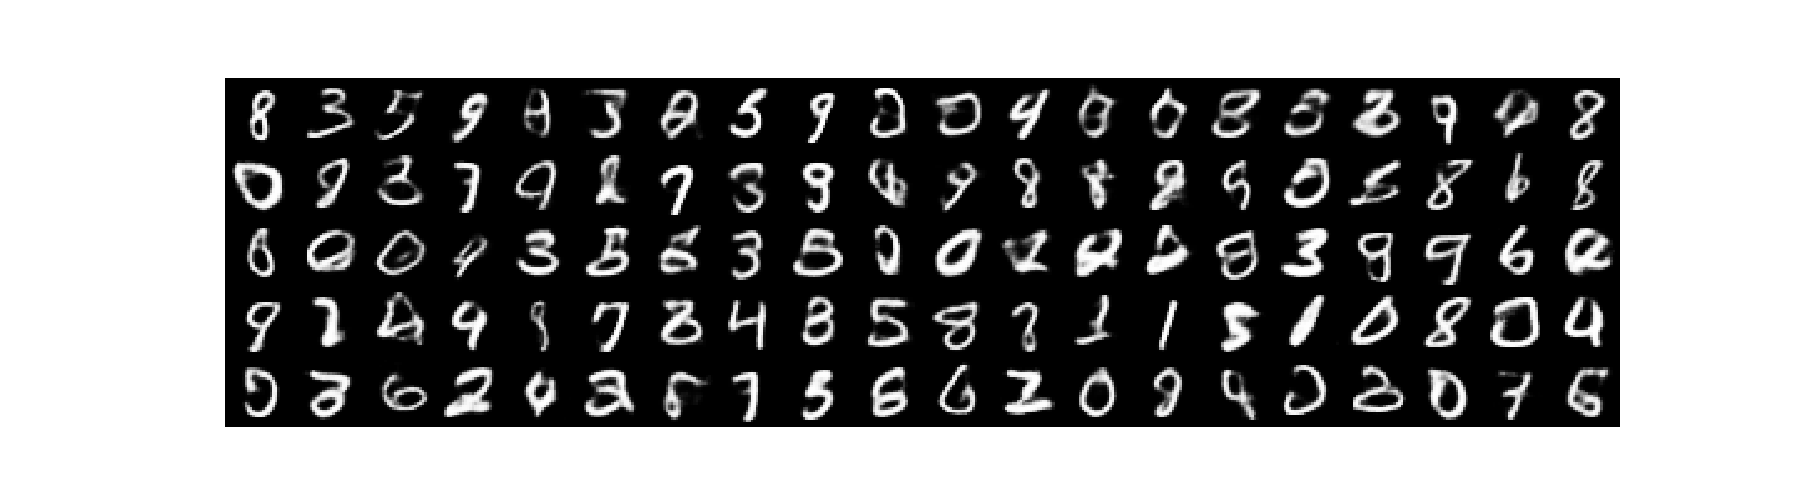
\includegraphics[width=\linewidth]{VAE_MNIST_0_100_256.png}
    \caption{\small Results on 3 hidden layers} \label{fig:a}
    \end{subfigure}\hspace*{\fill}
    \begin{subfigure}{0.49\textwidth}
    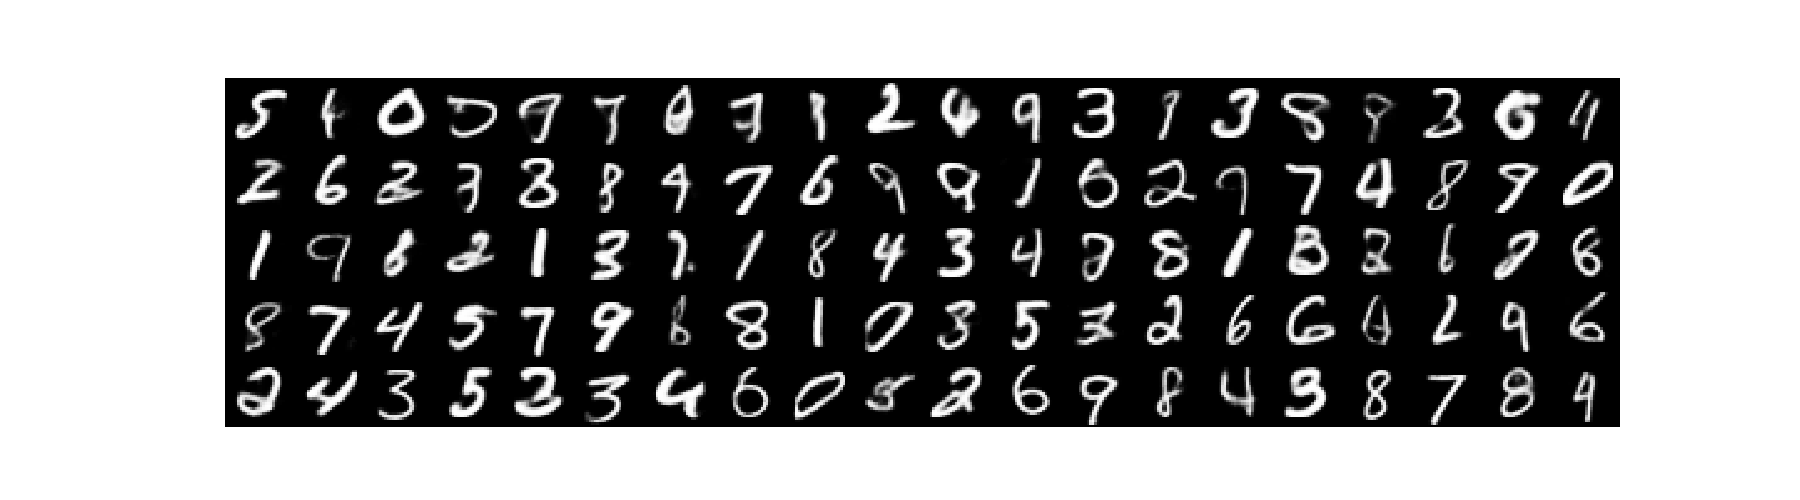
\includegraphics[width=\linewidth]{VAE_MNIST_2_100_256.png}
    \caption{\small Results on 5 hidden layers} \label{fig:b}
    \end{subfigure}
    \medskip
    \begin{subfigure}{0.49\textwidth}
    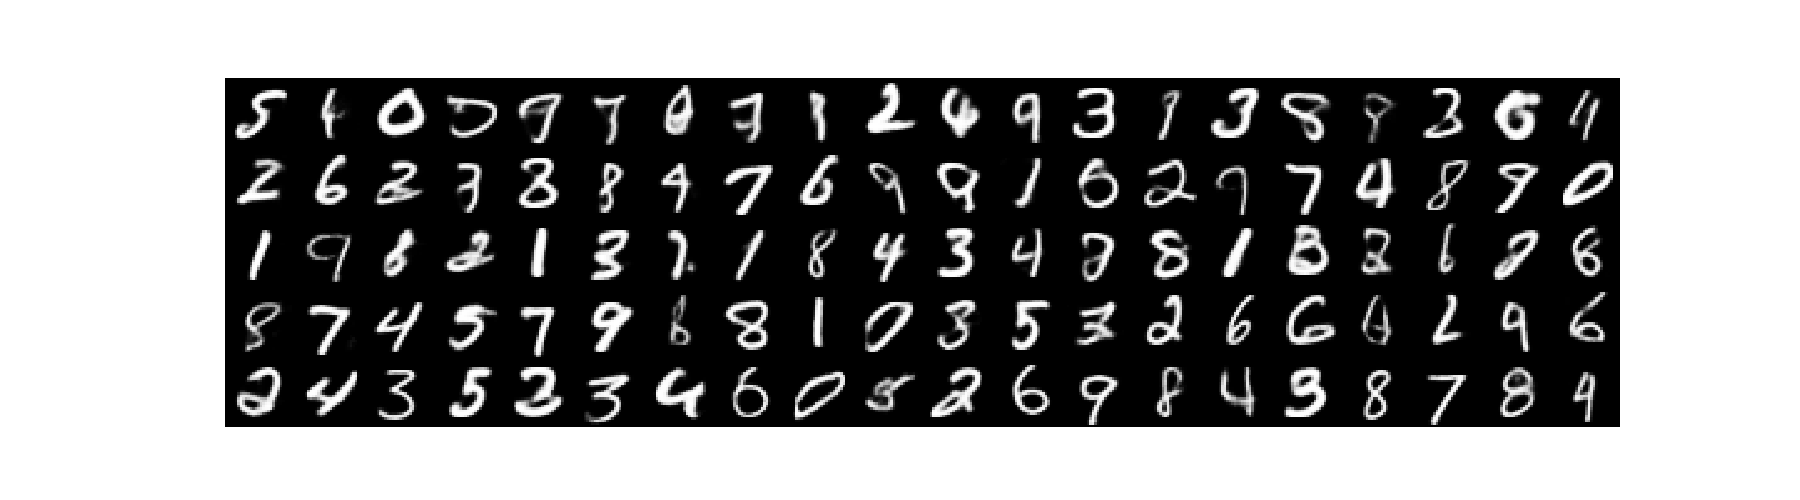
\includegraphics[width=\linewidth]{VAE_MNIST_2_100_256.png}
    \caption{\small Results on 5 hidden layers} \label{fig:c}
    \end{subfigure}
    \hspace*{\fill}
    \caption{Influence of the number of hidden layers on $3$ models, with performance increasing row by row} \label{fig:MNIST_VAE_hidden}
\end{figure}
% \begin{figure}[h]
%     \centering
%     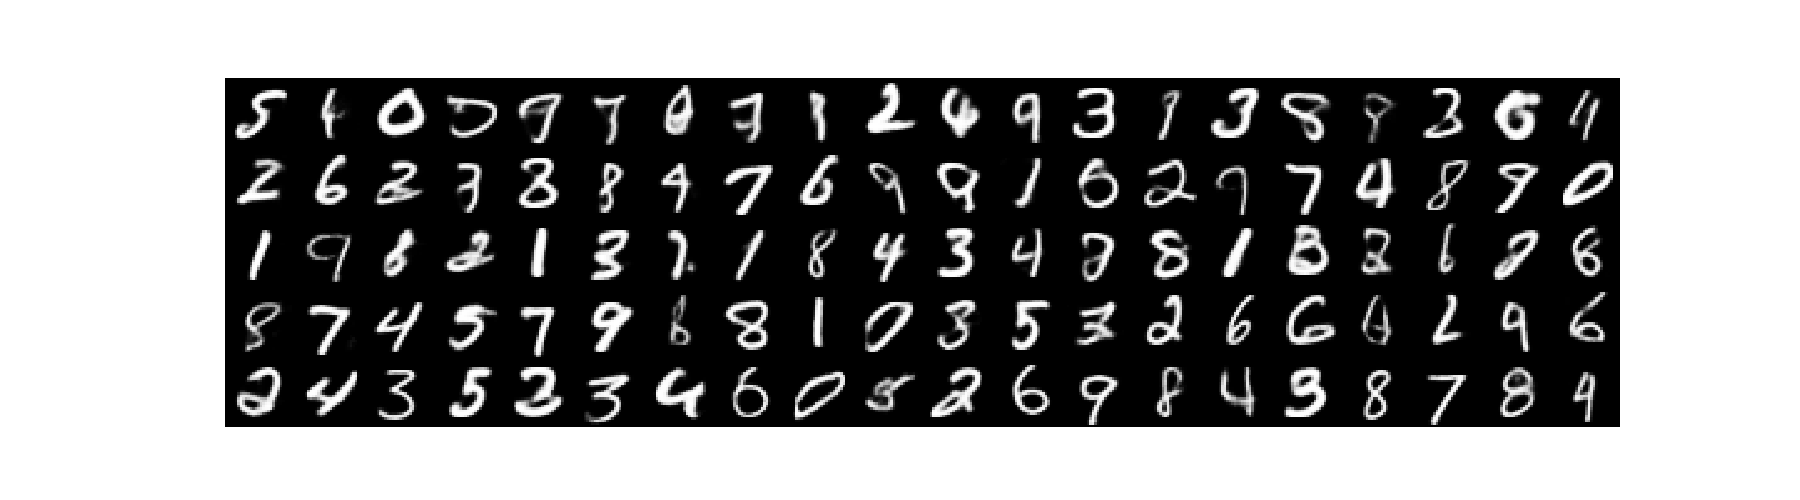
\includegraphics[width=.49\linewidth]{VAE_MNIST_2_100_256.png}
%     % \caption{\small Different latent size.}
%     % \label{fig:vae_latent}
% \end{figure}

In this homework, we used 3 hidden layers as the base model, and selectively add some convolutional layers with stride $(1, 1)$ in the middle of some $(2, 2)$ strides convolutional layers. 
\begin{figure}[h]
    \centering
    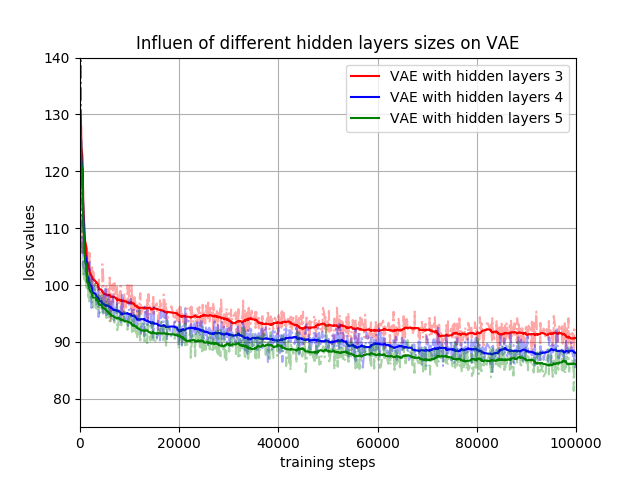
\includegraphics[width=.6\linewidth]{VAE_MNIST_hidden.png}
    \caption{\small Different number of hidden layers.}
    \label{fig:vae_hidden}
\end{figure}

% Intuitively, 5 hidden layers gets the better result than others. So, adding hidden layers can improve the performance of the model in this case, but too much hidden layers will lead to over-fitting.

In order to compare the training effort of the VAE model on different number of hidden layers, a plot of generator loss function value is created and plotted as Figure ~\ref{fig:vae_hidden}

A brief conclusion is drawn as follow,
\begin{itemize}
    \item The loss value of VAE with hidden layers 5 is the lowest, which means VAE with hidden layers 5 learnt better than models with other hidden layers.
    \item This implies more layers can help the model learn better.
\end{itemize}

\subsection{GAN}
\subsubsection{Latent Size}
First of all, let us take a look at generated good results, which are shown as Figure ~\ref{fig:MNIST_GAN_latent_results}, and generated images quality of different training time steps. The results are shown as Figure ~\ref{fig:MNIST_GAN_latent}

\begin{figure}[h]
    \centering
    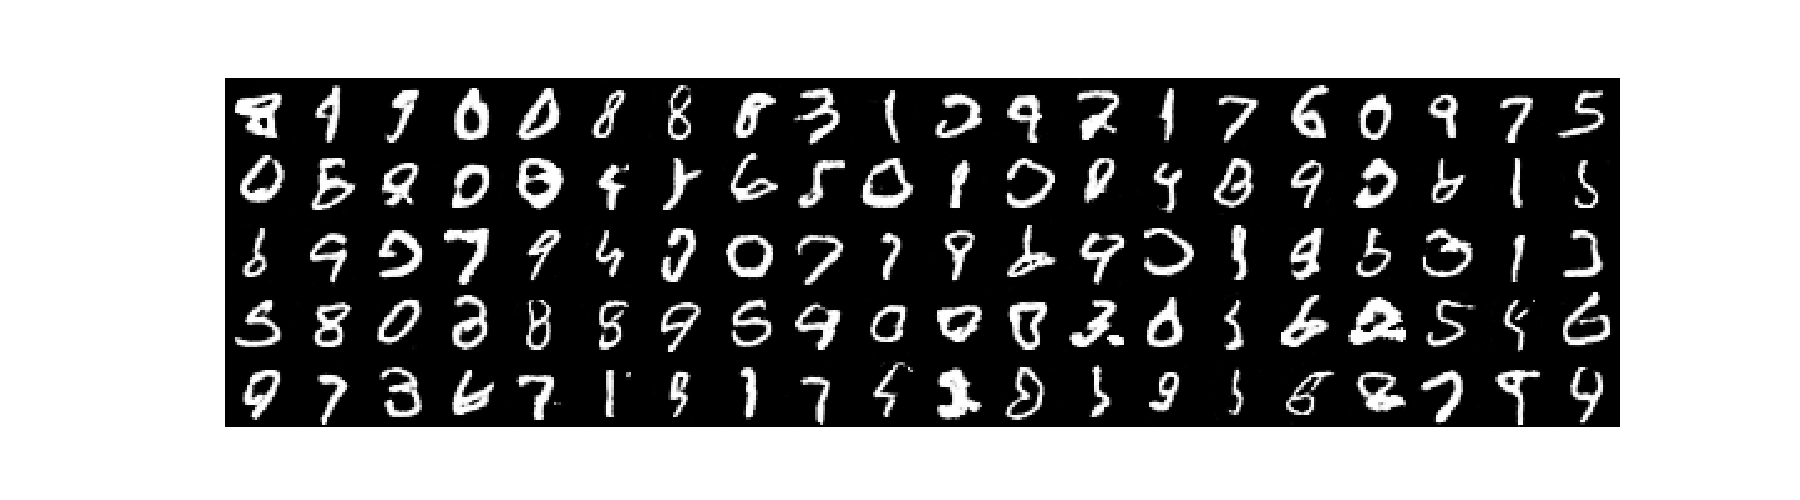
\includegraphics[width=.6\linewidth]{GAN_MNIST_0_100_256results.png}
    \caption{\small A random sample with final results.}
    \label{fig:MNIST_GAN_latent_results}
\end{figure}

To compare the influence of latent size, we fixed the number of hidden layers is $3$, and then compare latent size 10,20,50,100 and 200.

\begin{figure}[h]
    \begin{subfigure}{0.49\textwidth}
    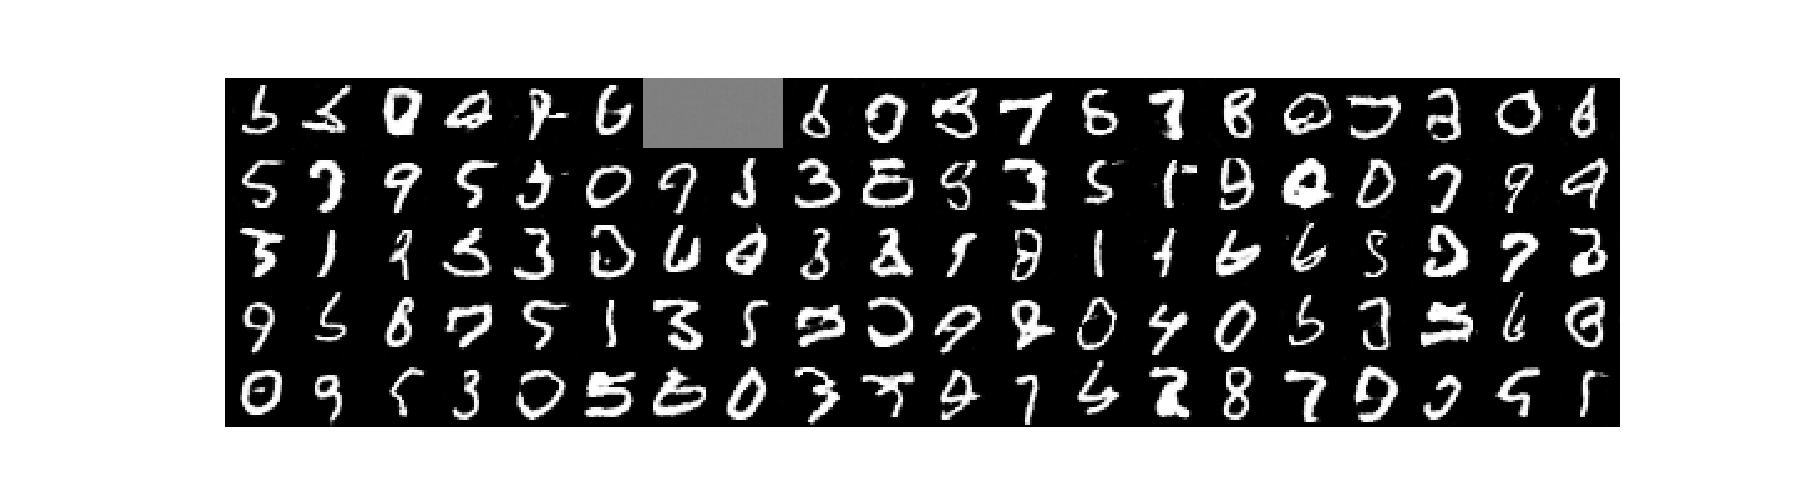
\includegraphics[width=\linewidth]{GAN_MNIST_0_10_256.png}
    \caption{\small Results on latent size 10.} \label{fig:a}
    \end{subfigure}\hspace*{\fill}
    \begin{subfigure}{0.49\textwidth}
    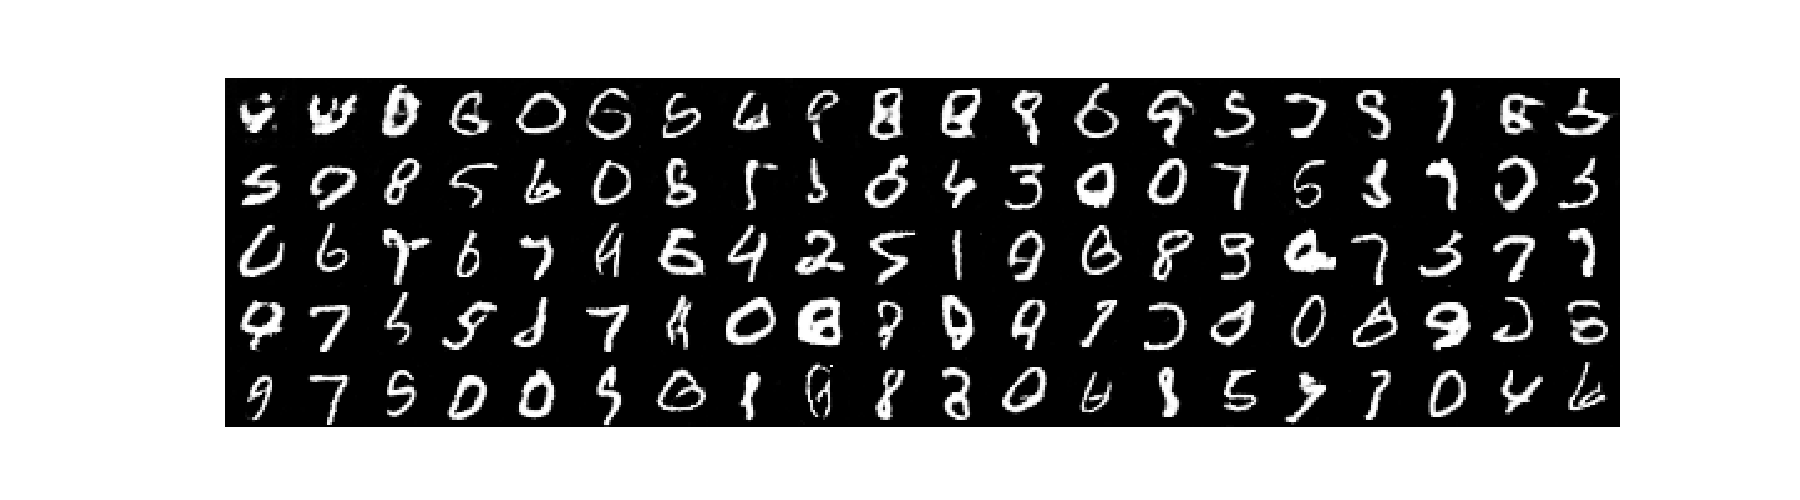
\includegraphics[width=\linewidth]{GAN_MNIST_0_20_256.png}
    \caption{\small Results on latent size 20.} \label{fig:b}
    \end{subfigure}
    
    \medskip
    \begin{subfigure}{0.49\textwidth}
    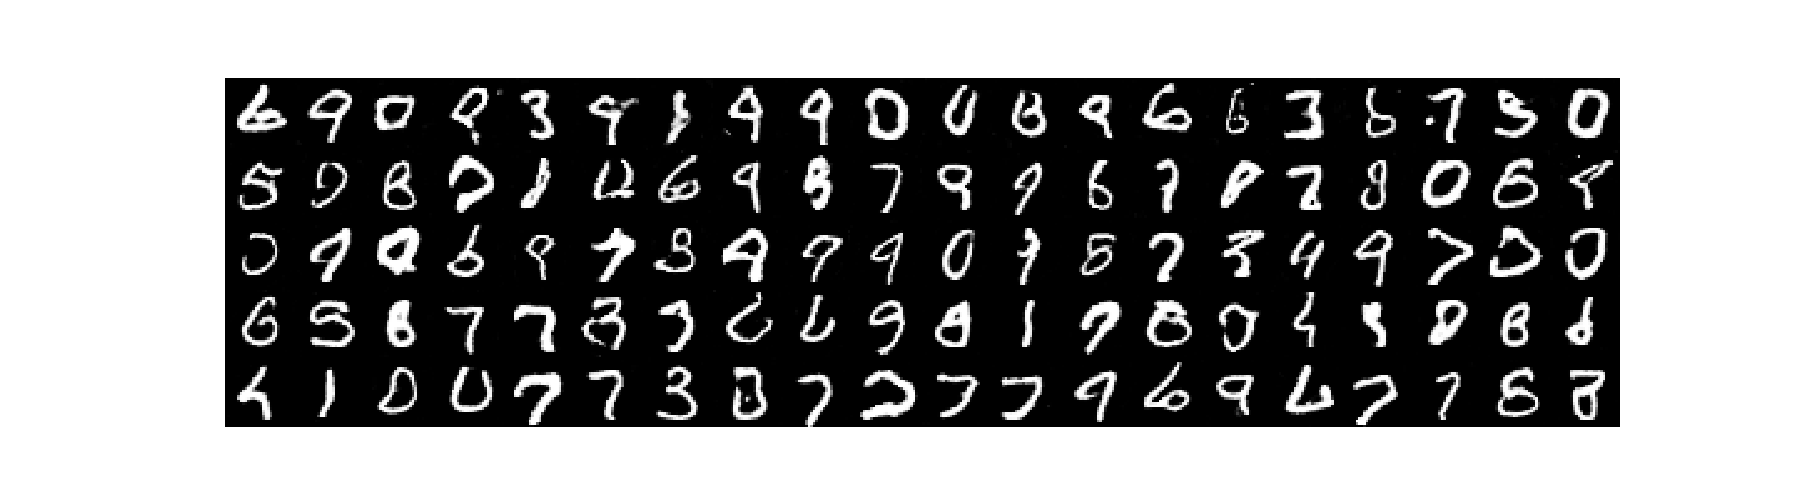
\includegraphics[width=\linewidth]{GAN_MNIST_0_50_256.png}
    \caption{\small Results on latent size 50.} \label{fig:c}
    \end{subfigure}\hspace*{\fill}
    \begin{subfigure}{0.49\textwidth}
    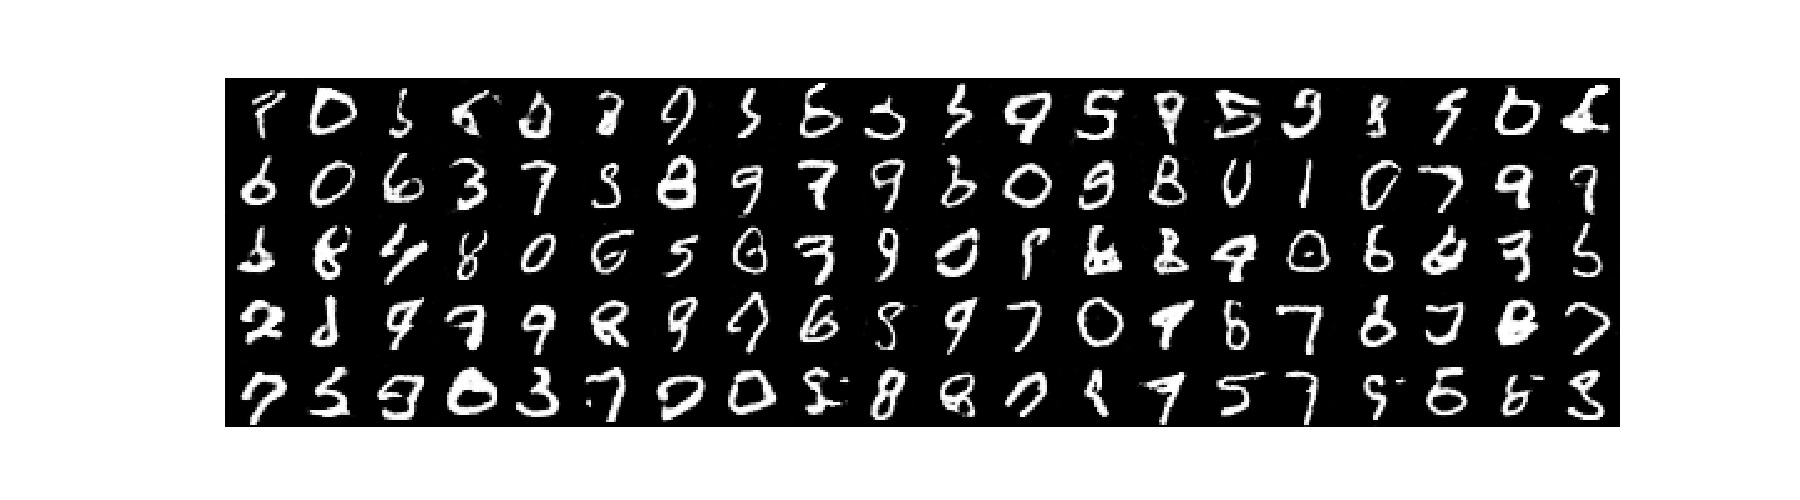
\includegraphics[width=\linewidth]{GAN_MNIST_0_100_256.png}
    \caption{\small Results on latent size 100.} \label{fig:d}
    \end{subfigure}
    
    % \medskip
    % \begin{subfigure}{0.49\textwidth}
    % 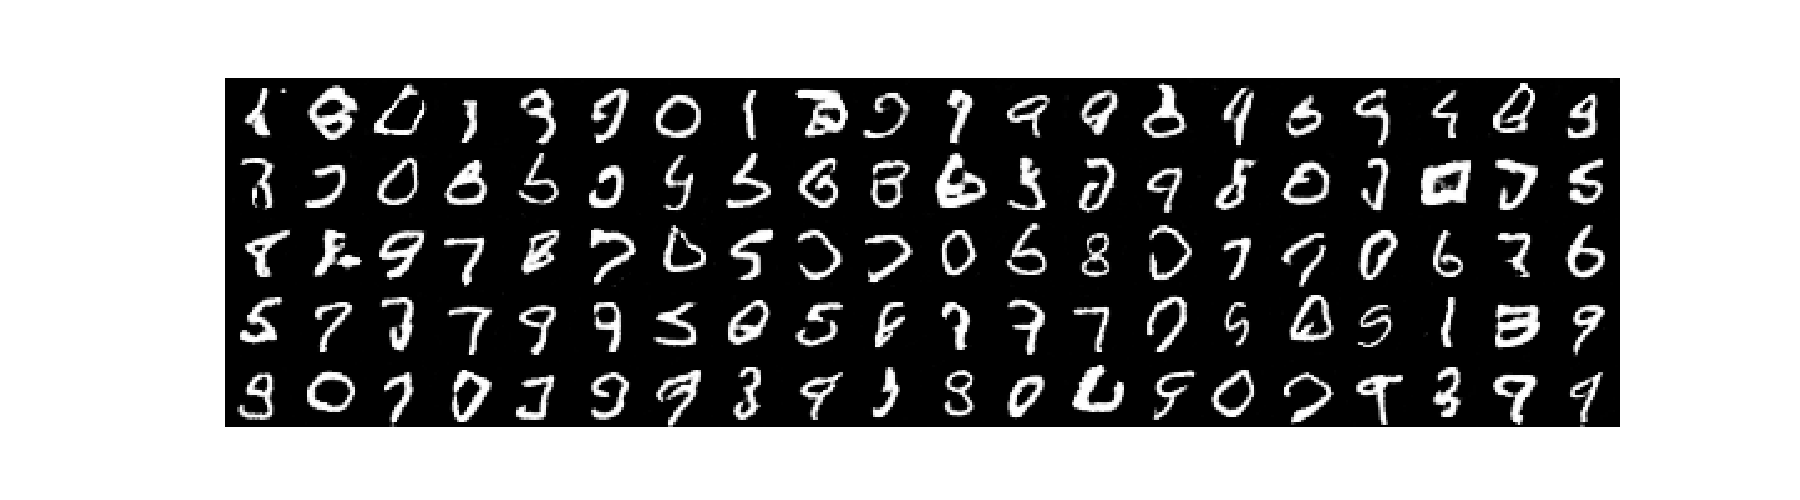
\includegraphics[width=\linewidth]{GAN_MNIST_0_200_256.png}
    % \caption{\small Results on latent size 200.} \label{fig:c}
    % \end{subfigure}
    \hspace*{\fill}
    \caption{Influence of the latent size on $5$ models, with performance increasing row by row} \label{fig:MNIST_GAN_latent}
\end{figure}

Intuitively, latent size 100 gets the better result than others. Similarly, too small or too large latent size will reduce the performance of GAN, there is the best result we can get when tuning latent size, and latent size is one of the key hyper-parameters which have to be tuned in real applications.

In order to compare the training effort of the GAN model on different latent space sizes, a plot of generator loss function value is created and plotted as Figure ~\ref{fig:gen_latent}
\begin{figure}[h]
    \centering
    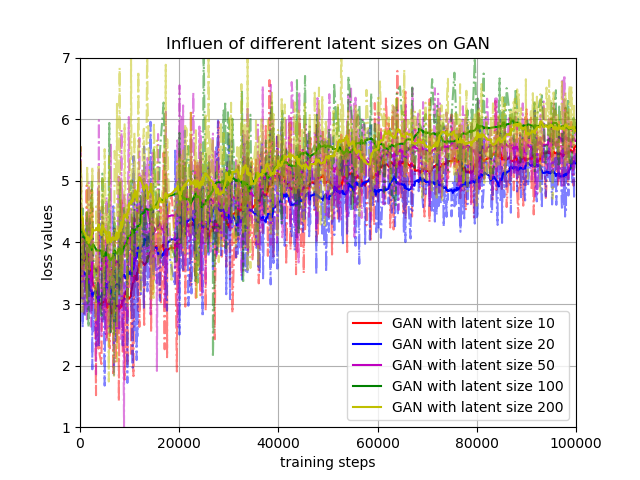
\includegraphics[width=.6\linewidth]{GAN_MNIST_latents.png}
    \caption{\small Different latent size.}
    \label{fig:gen_latent}
\end{figure}



A brief conclusion is drawn as follow,
\begin{itemize}
    \item From the overall view, increasing the latent size of generator in GAN will increase the performance
    \item However, the plot shows the performance of latent size 20 is the worst(lowest loss value) and latent size 100 is the best(highest loss value) in this experiment. But the loss value is still increasing, meaning the models have not completely converged yet. Our epochs are only 500, it is not sufficient to say which latent size can generate best images finally.
\end{itemize}
 


\subsubsection{Number of Hidden Layers}

First of all, let us take a look at the good quality results, which are shown as Figure ~\ref{fig:MNIST_GAN_hidden_results}, and increasing quality results are shown as Figure ~\ref{fig:MNIST_GAN_hidden}.

To compare the influence of the number of hidden layers, we fixed the latent size is $100$, and then compare the number of hidden layers 3,4 and 5.

\begin{figure}[h]
    \centering
    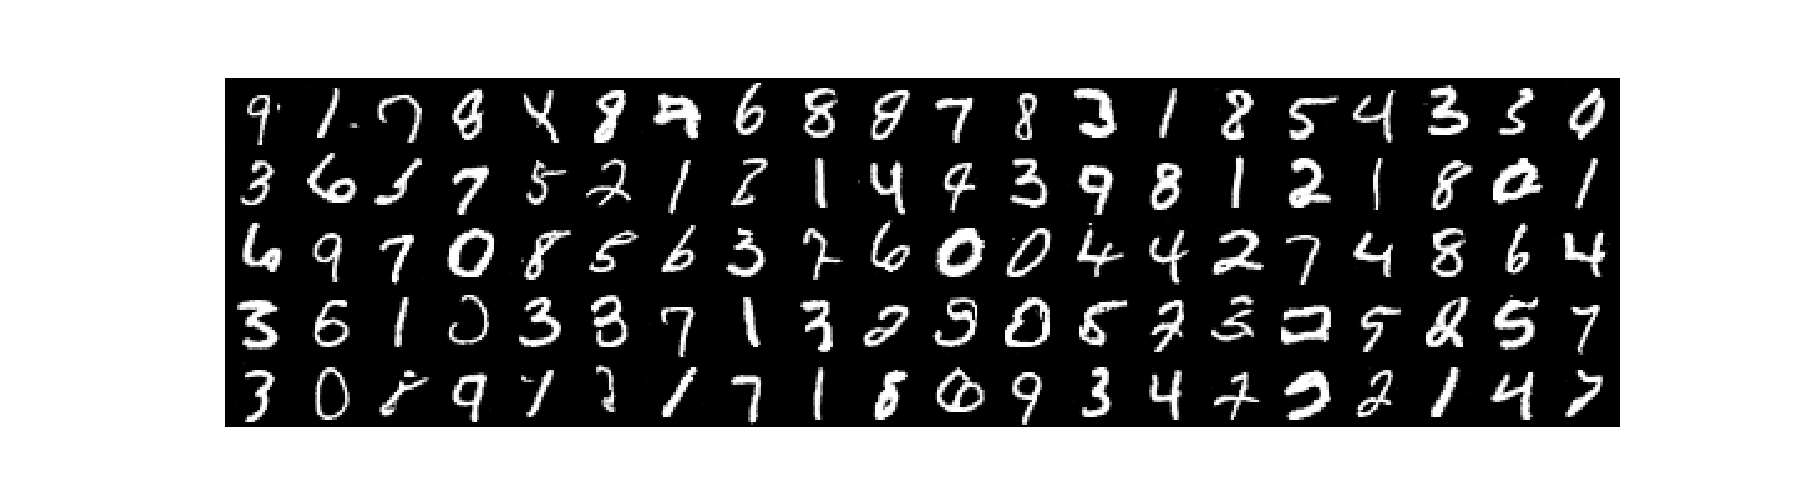
\includegraphics[width=.6\linewidth]{GAN_MNIST_2_100_256results.png}
    \caption{\small A random sample with final results.}
    \label{fig:MNIST_GAN_hidden_results}
\end{figure}

\begin{figure}[h]
    \begin{subfigure}{0.49\textwidth}
    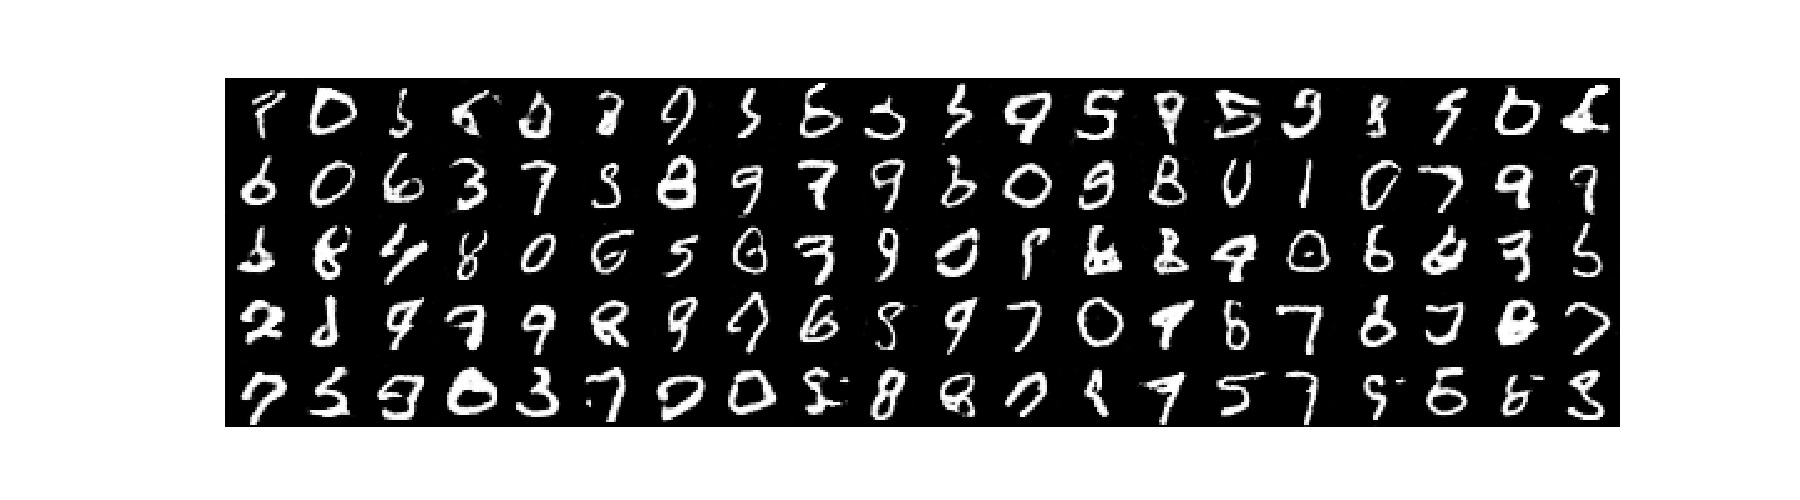
\includegraphics[width=\linewidth]{GAN_MNIST_0_100_256.png}
    \caption{\small Results on 3 hidden layers} \label{fig:a}
    \end{subfigure}\hspace*{\fill}
    \begin{subfigure}{0.49\textwidth}
    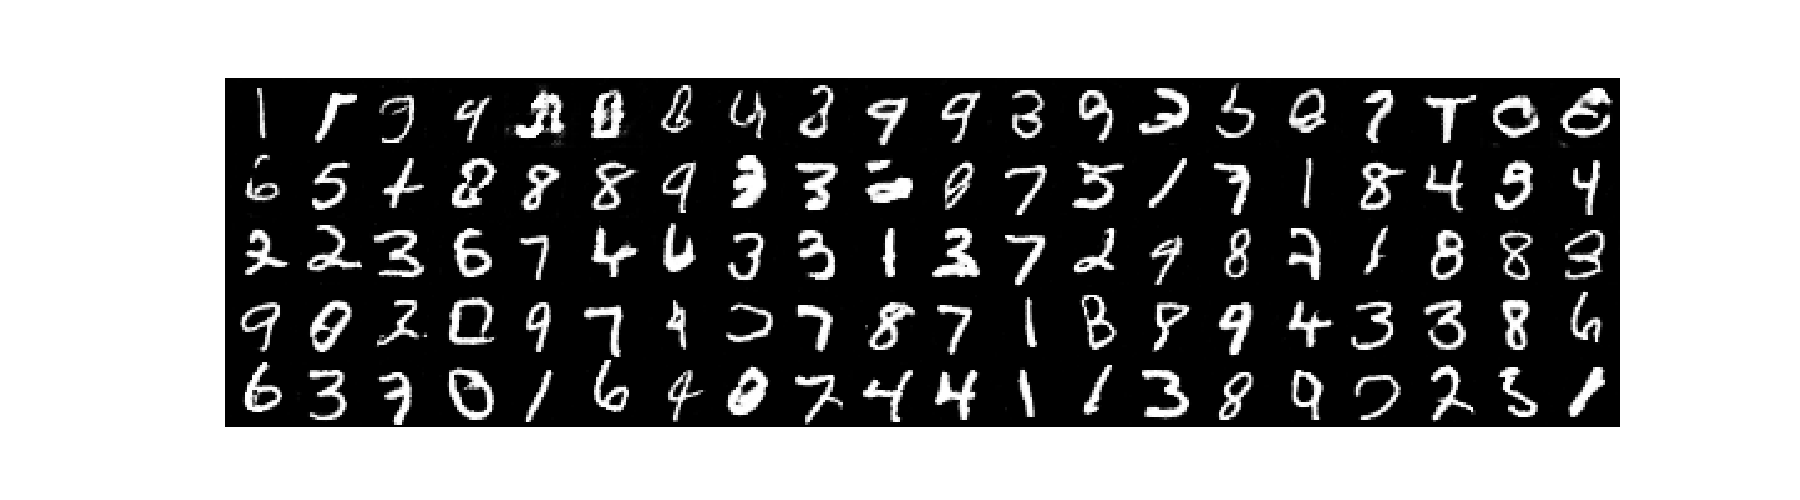
\includegraphics[width=\linewidth]{GAN_MNIST_1_100_256.png}
    \caption{\small Results on 4 hidden layers} \label{fig:b}
    \end{subfigure}

    \medskip
    \begin{subfigure}{0.49\textwidth}
    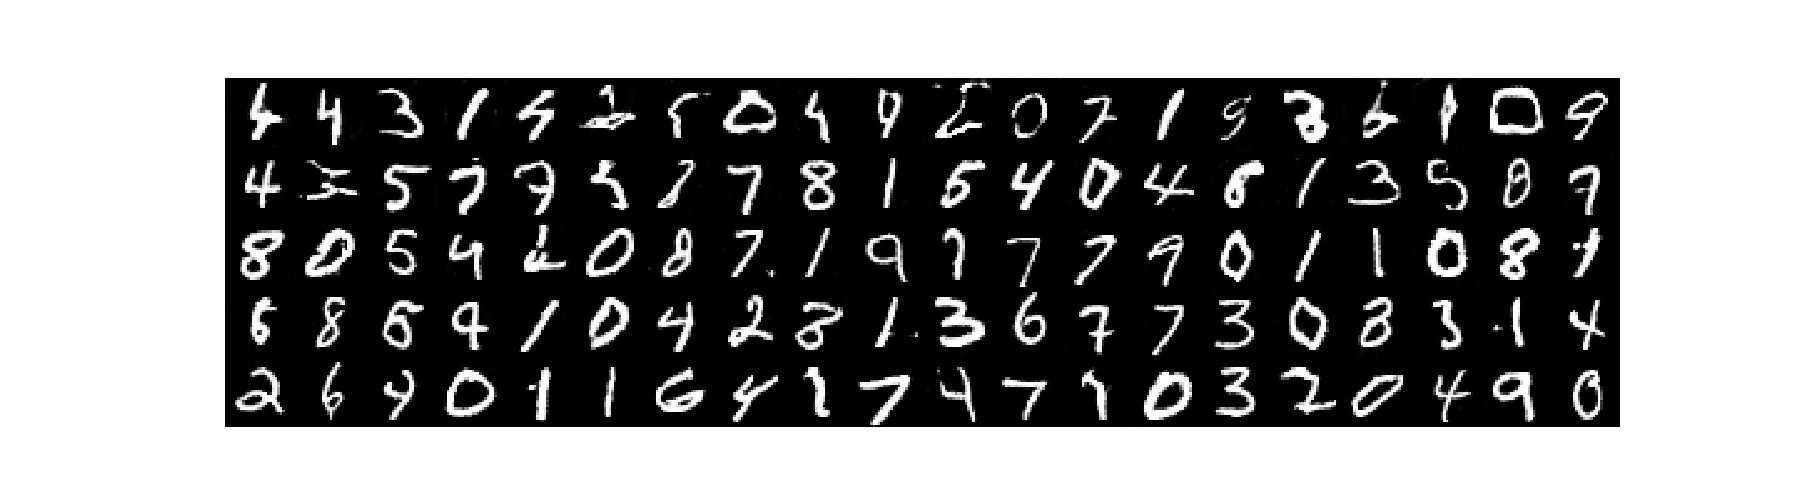
\includegraphics[width=\linewidth]{GAN_MNIST_2_100_256.png}
    \caption{\small Results on 5 hidden layers} \label{fig:c}
    \end{subfigure}\hspace*{\fill}
    \caption{Influence of the number of hidden layers on $3$ models, with performance increasing row by row} \label{fig:MNIST_GAN_hidden}
\end{figure}

A plot of generator loss function value is created and plotted as Figure ~\ref{fig:gen_hidden}
\begin{figure}[h]
    \centering
    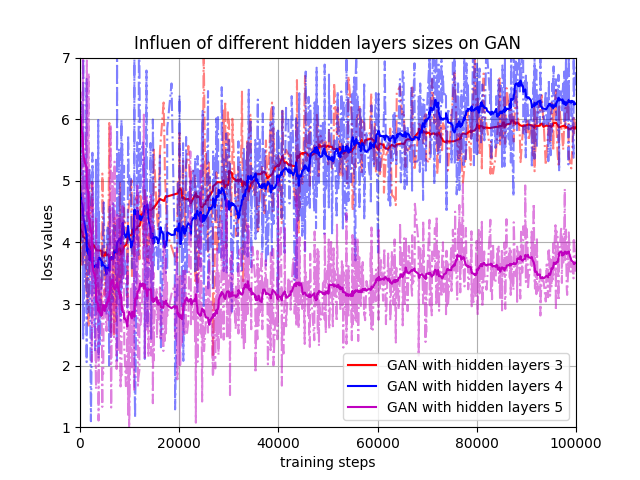
\includegraphics[width=.6\linewidth]{GAN_MNIST_hidden.png}
    \caption{\small Different number of hidden layers.}
    \label{fig:gen_hidden}
\end{figure}


A brief conclusion is drawn as follow,
\begin{itemize}
    \item From the figure, it is easy to tell the training efforts basically follow what we learnt from the lecture, that is, the JSD loss (represeted as generator loss) of GAN increases until it converges. This is the key feature that tells us whether the GAN is learning or not.
    \item One can notice that the overall performances of GAN on $3$ and $4$ layers are quite similar, but is worse on $5$ layers. This may lead to the conclusion that with increasing the hidden layers of the GAN model, it will dampen the model performance. However, another explanation may also be corret: Since the model has more weights to train, it may take time to learn. But we only trained the model on $1000$ epochs, it may not be sufficient to say "more layers, worse performance".
    \item Although the performances of GAN on $3$ and $4$ layers show some similarities, one can still find out that at the last few epochs, $4$ layers GAN outperforms $3$ layers model. This may imply that within certain number of layers, the final performance would be better when we increase the model complexity.
\end{itemize}

% \textbf{Hyper-parameters settings}: The hyper-parameters we used to get these results are shown as follow,
% \begin{table}[h]
%         \centering
%         \vspace{\baselineskip}
%         \caption{All relative parameters values.}\label{T:parameters}
%       \begin{tabular}{cc}
%         \hline
%         Parameter & Value\\
%         \hline
%         learning rate & 0.0001\\
%         optimizer & Adam\\
%         \hline
%       \end{tabular}
% \end{table}
%%%%%%%%%%%%%%%%%%%%%%%%%%%%%%%%%%%%%%%%%%%%%%%%%%%%
\subsection{WGAN}

The difference of GAN and WGAN is cost function, and they use different cost function to find the optimal solution. So converting GAN to WGAN needs $3$ operations:
\begin{itemize}
    \item Remove sigmoid activation function of the last dense layer in discriminator
    \item Change loss function of both generator and discriminator
    \item Use weight clip when updating the weight or gradient penalty, which is called WGAN-GP.
\end{itemize}

\subsubsection{Latent Size}

First of all, let us take a look at the good quality results, which are shown as Figure ~\ref{fig:MNIST_WGAN_latent_results} and increasing quality results are shown as Figure ~\ref{fig:MNIST_WGAN_latent}.
\begin{figure}[h]
    \centering
    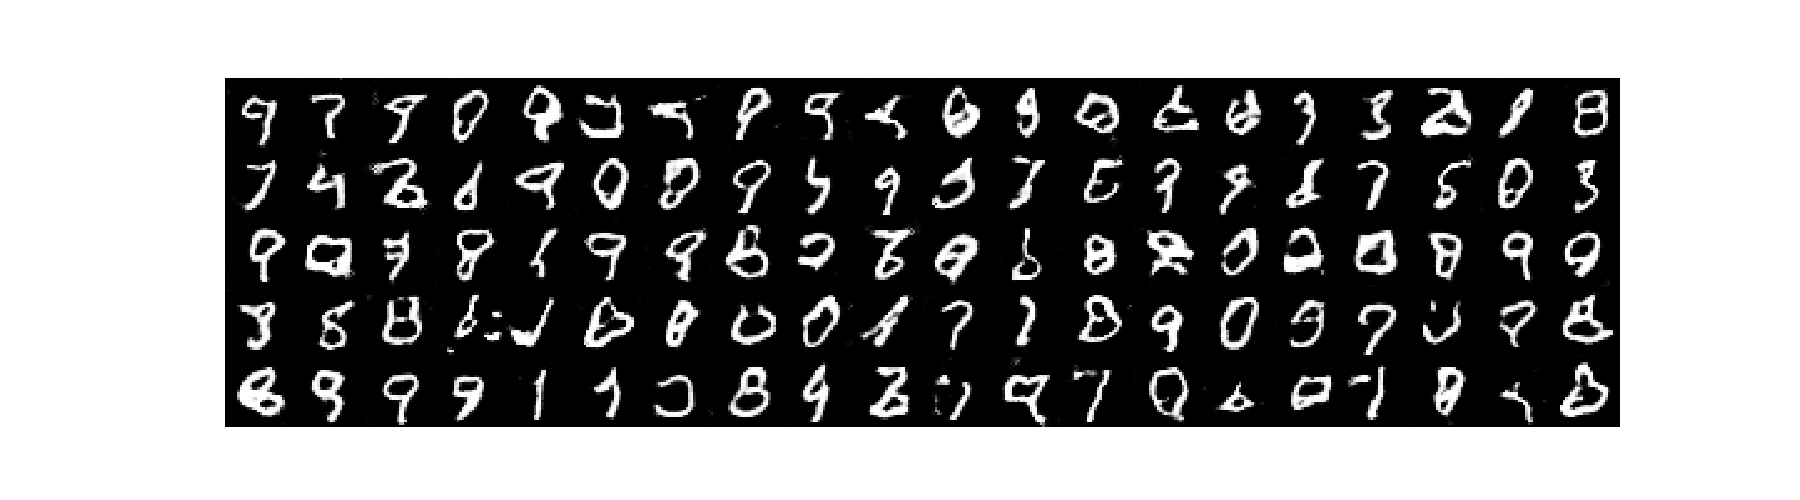
\includegraphics[width=.6\linewidth]{WGAN_MNIST_0_200_256results.png}
    \caption{\small A random sample with final results.}
    \label{fig:MNIST_WGAN_latent_results}
\end{figure}

\begin{figure}[h]
    \begin{subfigure}{0.49\textwidth}
    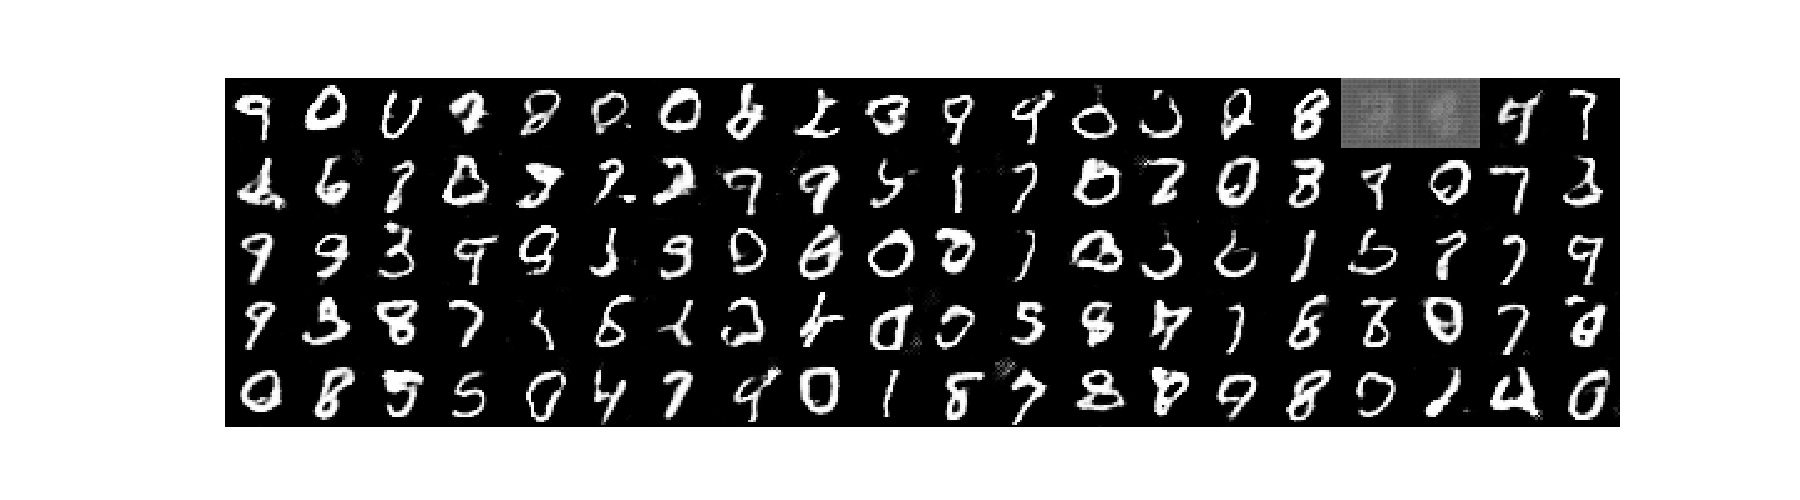
\includegraphics[width=\linewidth]{WGAN_MNIST_0_10_256.png}
    \caption{\small Results on latent size 10.} \label{fig:a}
    \end{subfigure}\hspace*{\fill}
    \begin{subfigure}{0.49\textwidth}
    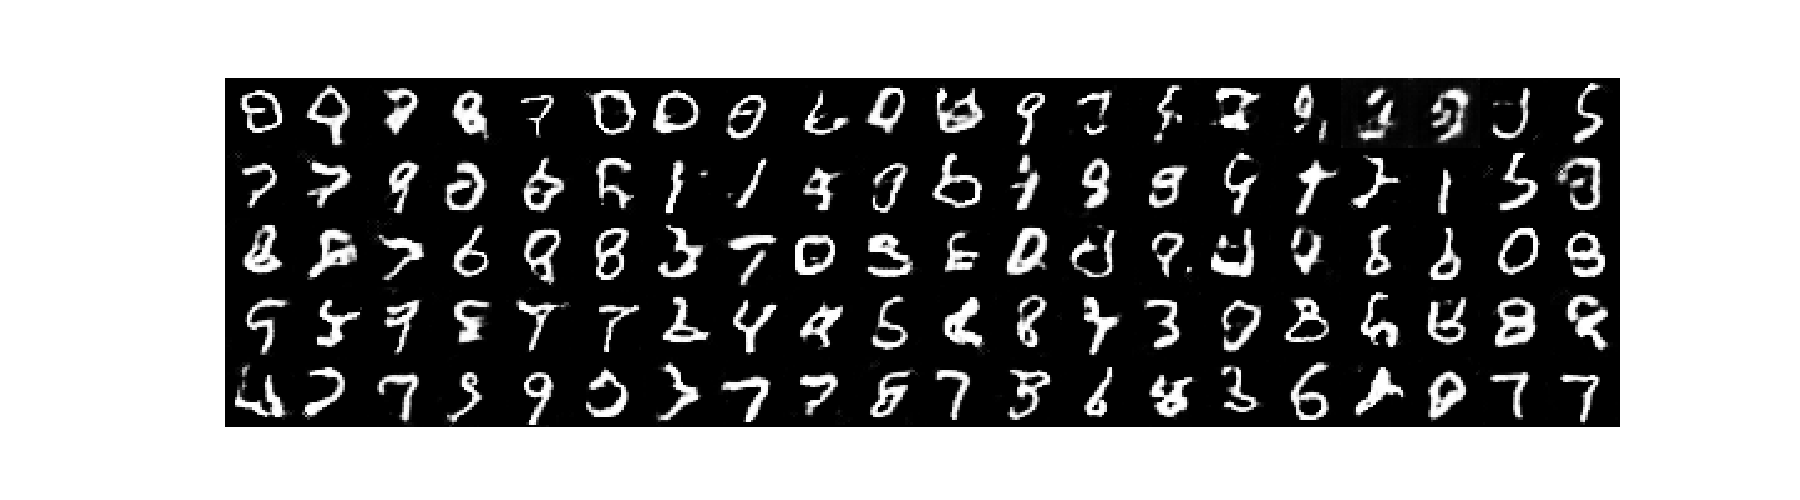
\includegraphics[width=\linewidth]{WGAN_MNIST_0_20_256.png}
    \caption{\small Results on latent size 20.} \label{fig:b}
    \end{subfigure}
    
    \medskip
    \begin{subfigure}{0.49\textwidth}
    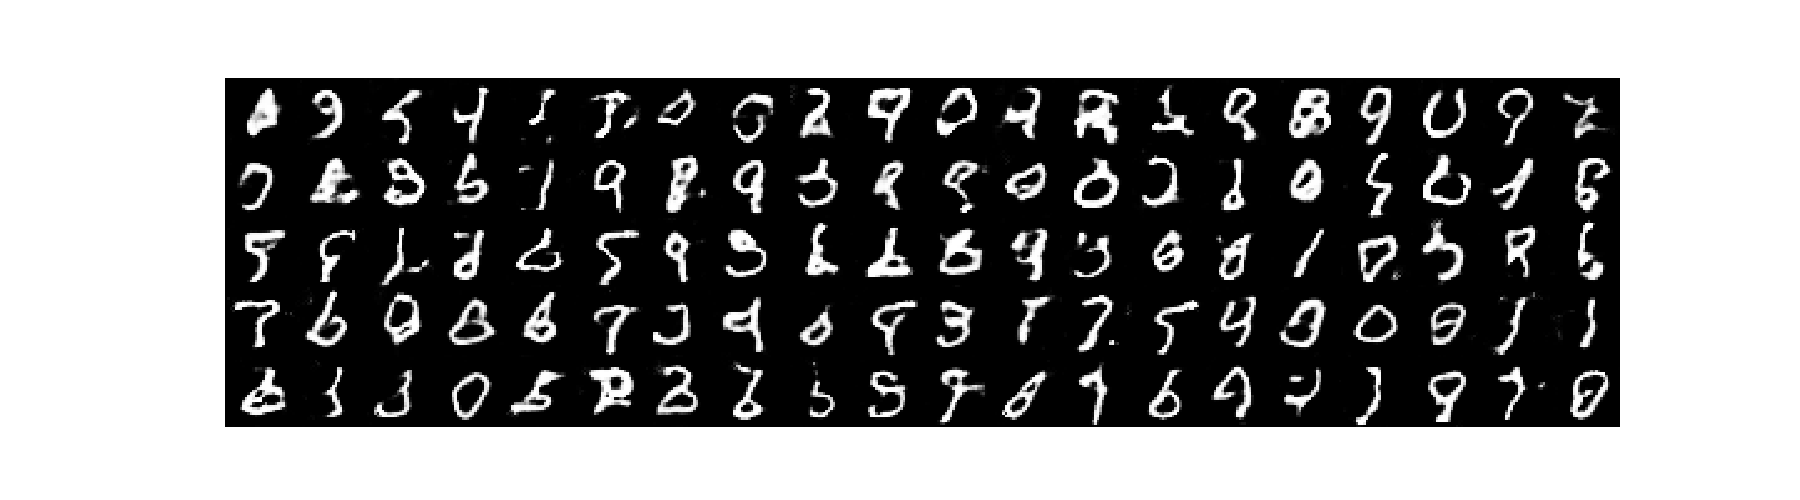
\includegraphics[width=\linewidth]{WGAN_MNIST_0_50_256.png}
    \caption{\small Results on latent size 50.} \label{fig:c}
    \end{subfigure}\hspace*{\fill}
    \begin{subfigure}{0.49\textwidth}
    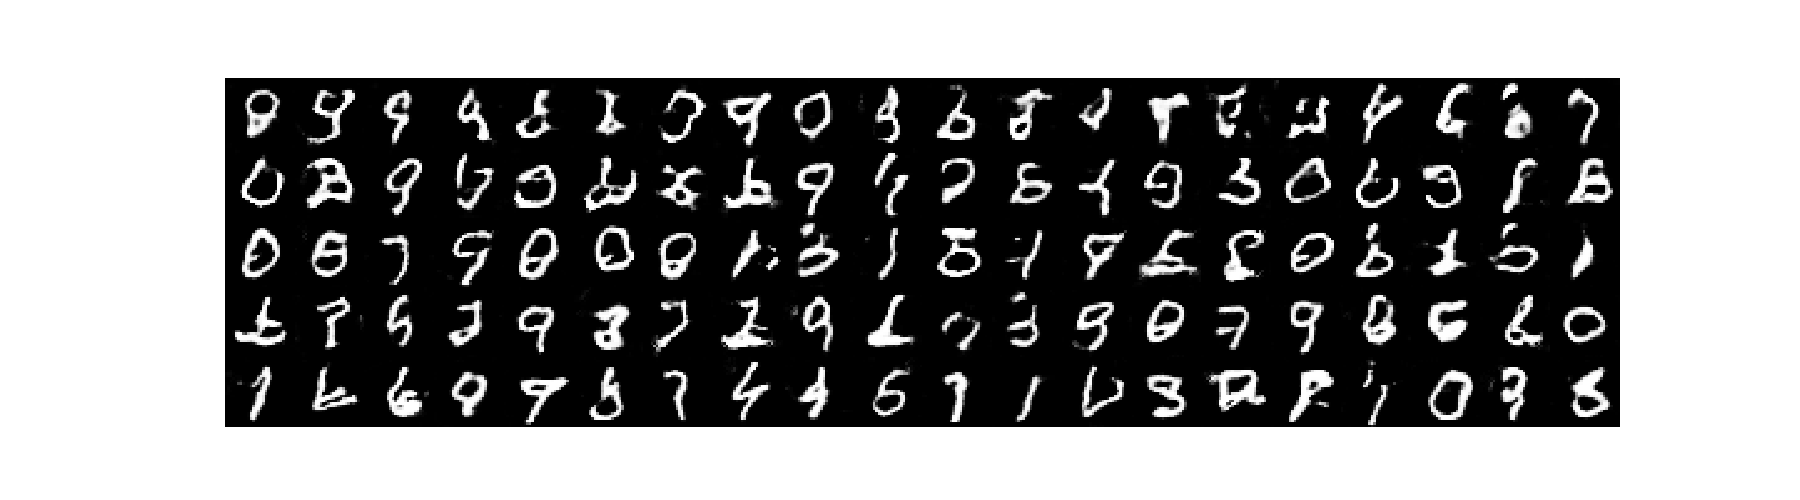
\includegraphics[width=\linewidth]{WGAN_MNIST_0_100_256.png}
    \caption{\small Results on latent size 100.} \label{fig:d}
    \end{subfigure}
    
    % \medskip
    % \begin{subfigure}{0.49\textwidth}
    % 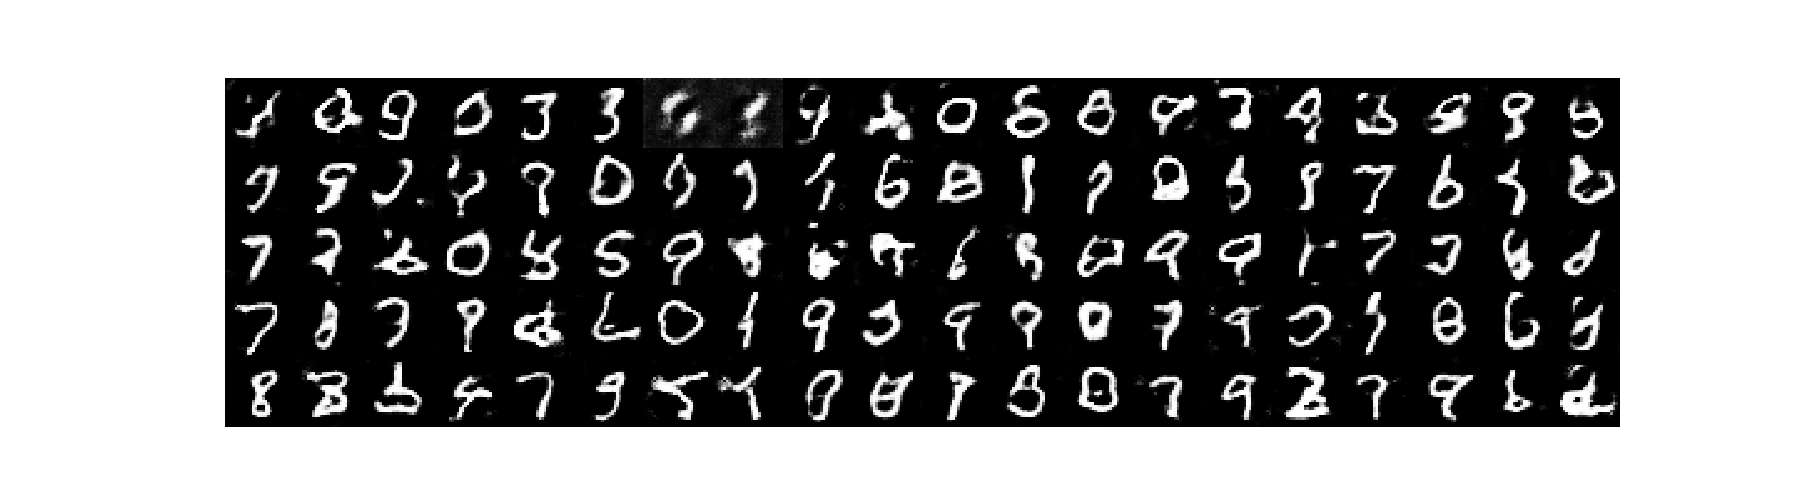
\includegraphics[width=\linewidth]{WGAN_MNIST_0_200_256.png}
    % \caption{\small Results on latent size 200.} \label{fig:c}
    % \end{subfigure}
    \hspace*{\fill}
    \caption{Influence of the latent size on $5$ models, with performance increasing row by row} \label{fig:MNIST_WGAN_latent}
\end{figure}

Here, latent size 10 gets the better result than others, which is different to the best latent size of GAN, so for each kind of GAN model, there is one matching best latent size to reach the best performance.

In order to compare the training effort of the WGAN model on different latent space sizes, a plot of generator loss function value is created and plotted as Figure ~\ref{fig:wgen_latent}
\begin{figure}[h]
    \centering
    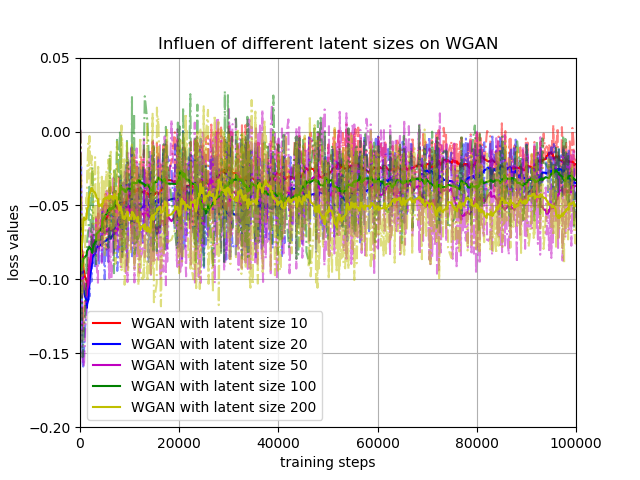
\includegraphics[width=.6\linewidth]{WGAN_MNIST_latents.png}
    \caption{\small Different latent size.}
    \label{fig:wgen_latent}
\end{figure}



A brief conclusion is drawn as follow,
\begin{itemize}
    \item The overall training processes agree with the curve we learnt from the lecture, with the training step goes up, the EMD loss (represented as generator loss) decreases.
    \item It is not hard to find that with the latent size increasing, the loss value becomes greater. This can generally be concluded as, increasing the latent size on the WGAN model (training on MNIST datasets) can worsen the final performance.
    \item The WGAN is easier to converge than GAN, but the final performance of WGAN is worse than GAN. 
\end{itemize}
 

\subsubsection{Number of Hidden Layers}

First of all, let us take a look at the good quality results, which are shown as Figure ~\ref{fig:MNIST_WGAN_hidden_results} and increasing quality results are shown as Figure ~\ref{fig:MNIST_WGAN_hidden}

Increasing number of hidden layers in both Critic and Generator simultaneously. 
\begin{figure}[h]
    \centering
    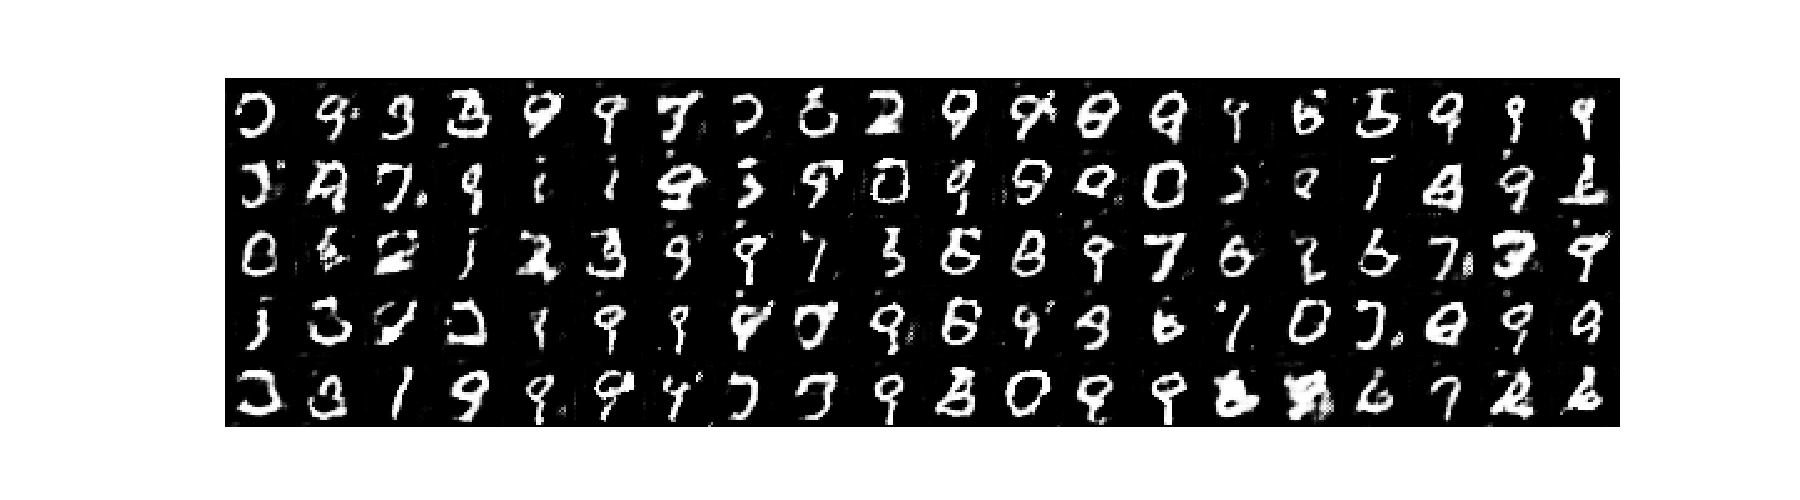
\includegraphics[width=.6\linewidth]{WGAN_MNIST_2_100_256results.png}
    \caption{\small A random sample with final results.}
    \label{fig:MNIST_WGAN_hidden_results}
\end{figure}

\begin{figure}[h]
    \begin{subfigure}{0.49\textwidth}
    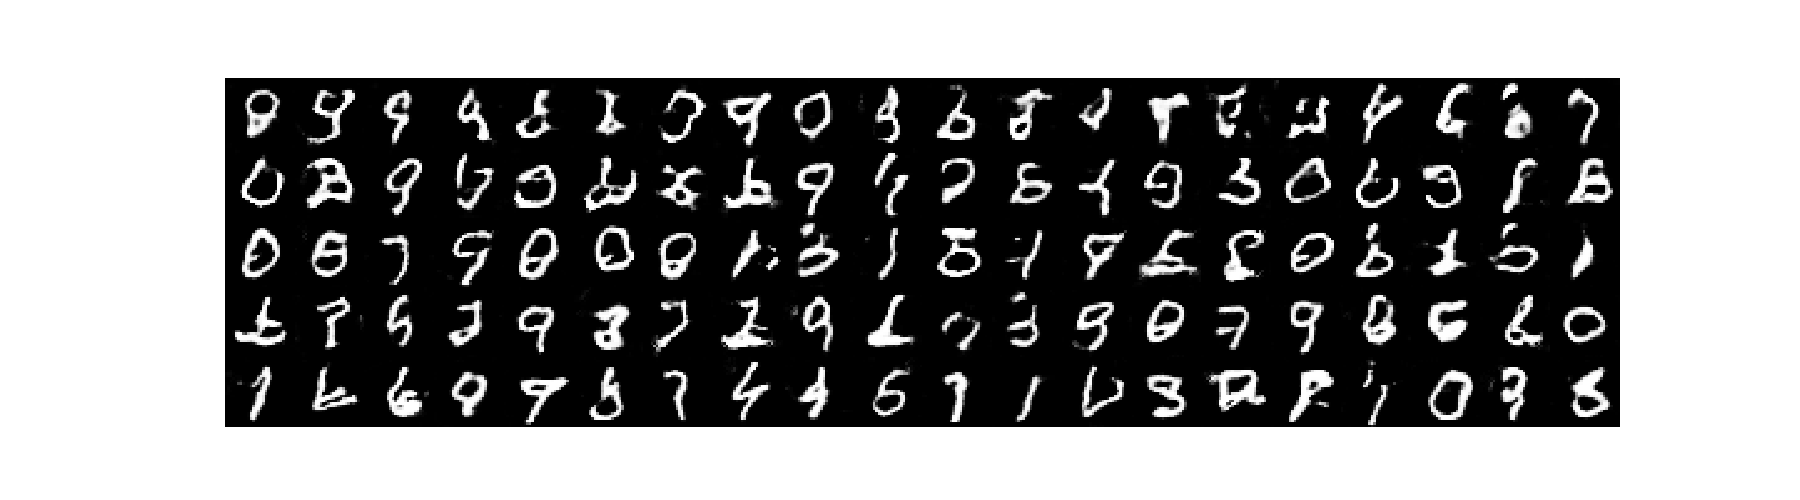
\includegraphics[width=\linewidth]{WGAN_MNIST_0_100_256.png}
    \caption{\small Results on 3 hidden layers} \label{fig:a}
    \end{subfigure}\hspace*{\fill}
    \begin{subfigure}{0.49\textwidth}
    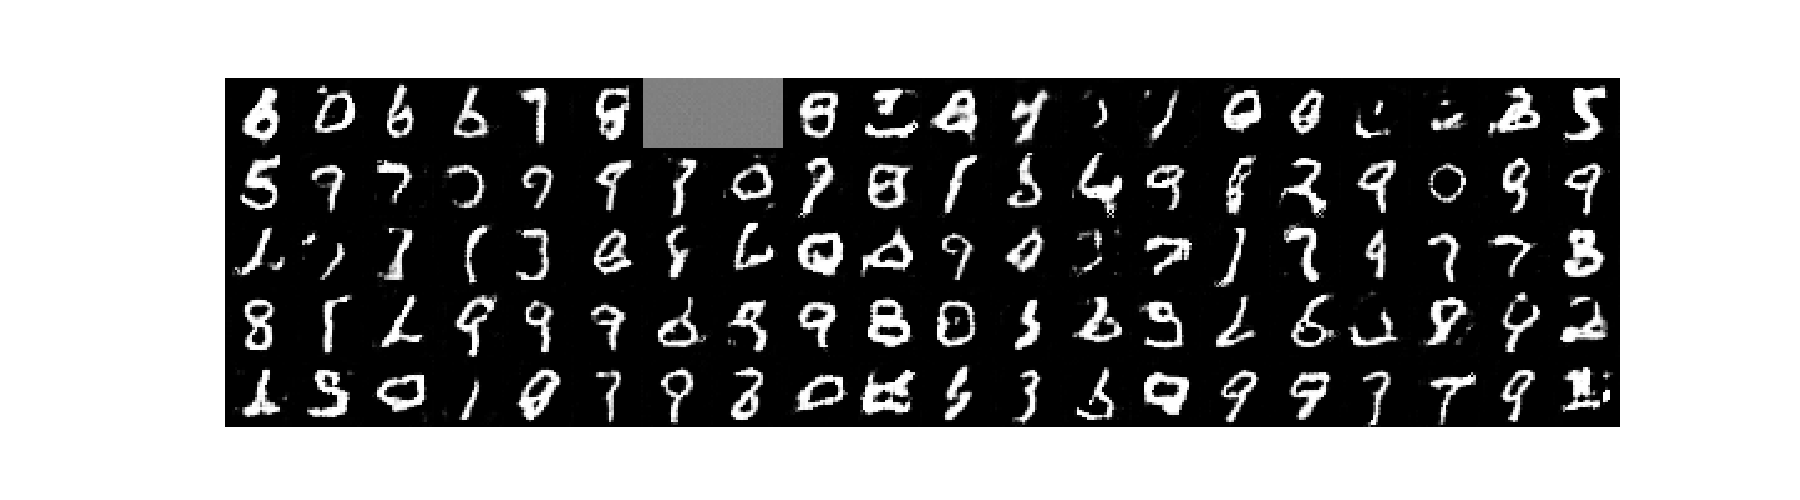
\includegraphics[width=\linewidth]{WGAN_MNIST_1_100_256.png}
    \caption{\small Results on 4 hidden layers} \label{fig:b}
    \end{subfigure}

    \medskip
    \begin{subfigure}{0.49\textwidth}
    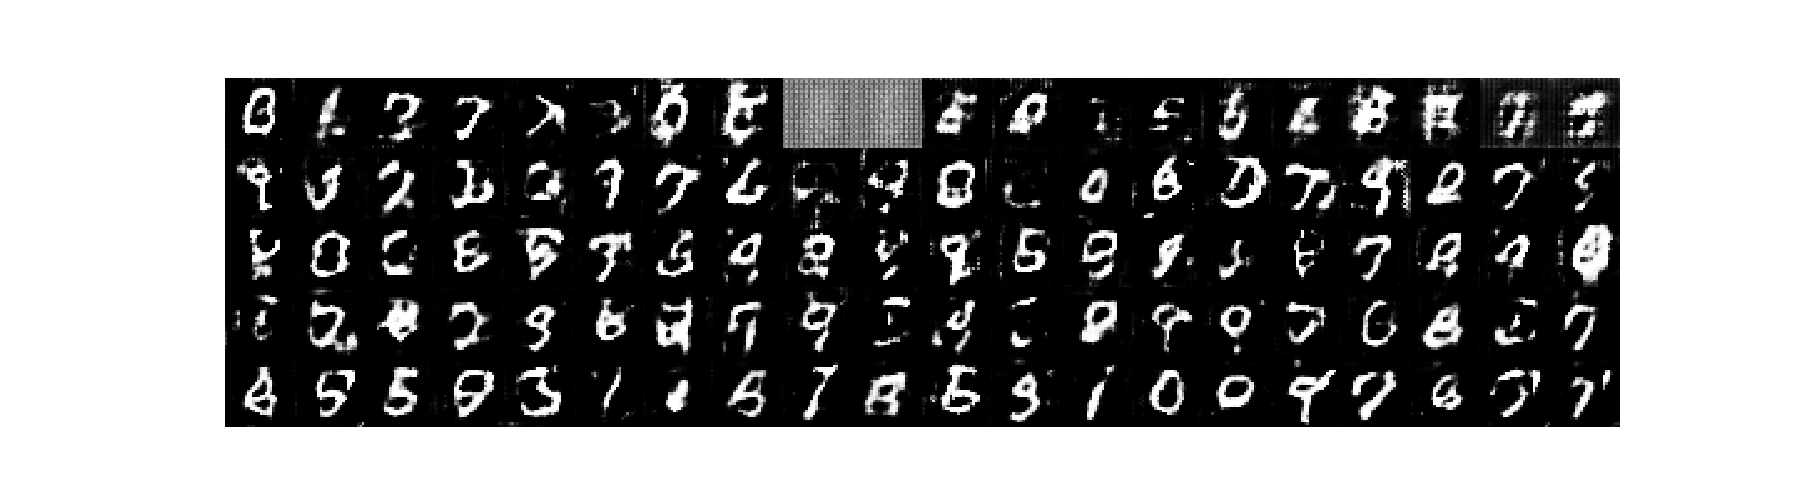
\includegraphics[width=\linewidth]{WGAN_MNIST_2_100_256.png}
    \caption{\small Results on 5 hidden layers} \label{fig:c}
    \end{subfigure}\hspace*{\fill}
    \caption{Influence of the number of hidden layers on $3$ models, with performance increasing row by row} \label{fig:MNIST_WGAN_hidden}
\end{figure}

Intuitively, 5 hidden layers gets the better result than others, which is different to the best number of hidden layers of GAN. So, for each kind of GAN model, there is one matching best number of hidden layers to reach the best performance.

In order to compare the training effort of the WGAN model on different number of hidden layers, a plot of generator loss function value is created and plotted as Figure ~\ref{fig:wgen_hidden}

\begin{figure}[h]
    \centering
    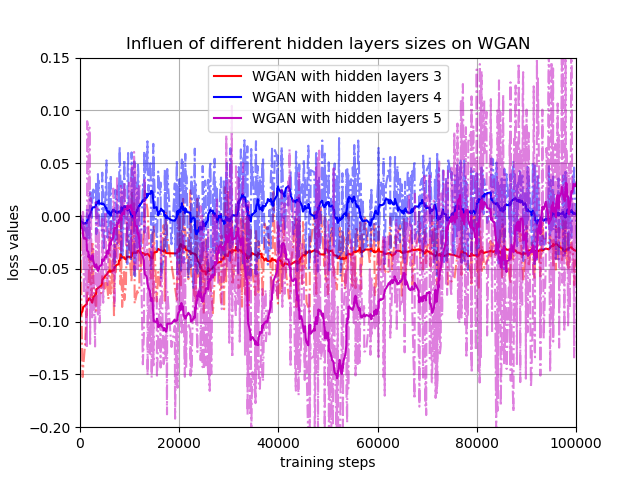
\includegraphics[width=.6\linewidth]{WGAN_MNIST_hidden.png}
    \caption{\small Different number of hidden layers.}
    \label{fig:wgen_hidden}
\end{figure}




A brief conclusion is drawn as follow,
\begin{itemize}
    \item Still, we can observe that the EMD loss is decreasing through the training process.
    \item By comparing the final performance of WGAN model on different hidden layers, we can say the more hidden layers the WGAN has, the better performance it will reach.
    \item It is easy to observe that the model becomes more unstable when we increase the hidden layers. The possible reason for this is that the implementation of WGAN itself is by clipping the weights. Since the more complex the model is, the more weights the model have to clip. As a result, it lead to changing the direction of weights frequently which is the main reason why the loss value fluctuates a lot.
\end{itemize}

% \textbf{Hyper-parameters settings}: The hyper-parameters we used to get these results are shown as follow,
% \begin{table}[h]
%         \centering
%         \vspace{\baselineskip}
%         \caption{All relative parameters values.}\label{T:parameters}
%       \begin{tabular}{cc}
%         \hline
%         Parameter & Value\\
%         \hline
%         learning rate & 0.00001\\
%         optimizer & RMSprop\\
%         weight clip & 0.01\\
%         \hline
%       \end{tabular}
% \end{table}


\section{CIFAR-10 Dataset}

Before dive into the content, we firstly have to apologize for the low quality of the generated images. We have tried several network structures and tuned hyper-parameters multi-times. Also, since the time is limited, we decided to set the training epochs as $1000$. The results we are currently presenting in this report is possibly the best we can get.

Back to the report, this section is separated into $3$ subsections with each model occupying one subsection.

\subsection{VAE}

\subsubsection{Latent Size}

First of all, let us take a look at the good quality results, which are shown as Figure ~\ref{fig:CIFAR_VAE_latent_results} 

\begin{figure}[h]
    \centering
    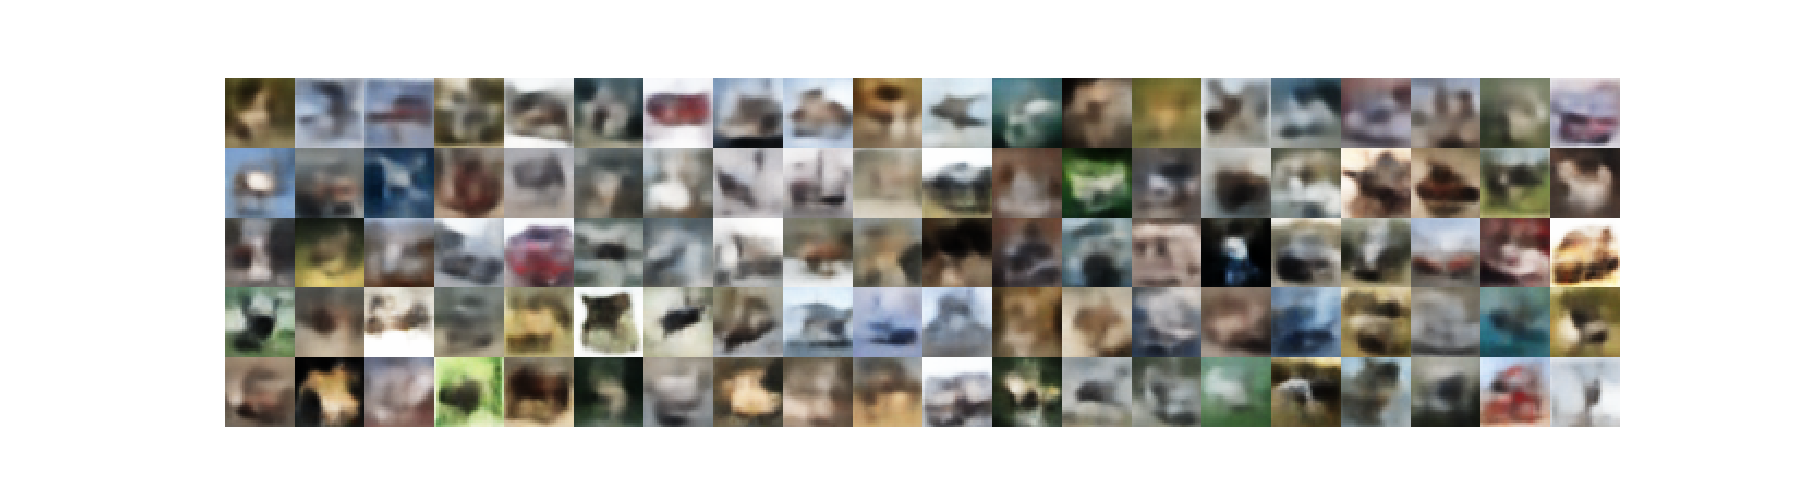
\includegraphics[width=.8\linewidth]{VAE_CIFAR_0_100_256.png}
    \caption{\small A random sample with final results.}
    \label{fig:CIFAR_VAE_latent_results}
\end{figure}

And increasing quality results are shown as Figure ~\ref{fig:CIFAR_VAE_latent}
\begin{figure}[h]
    \begin{subfigure}{0.495\textwidth}
    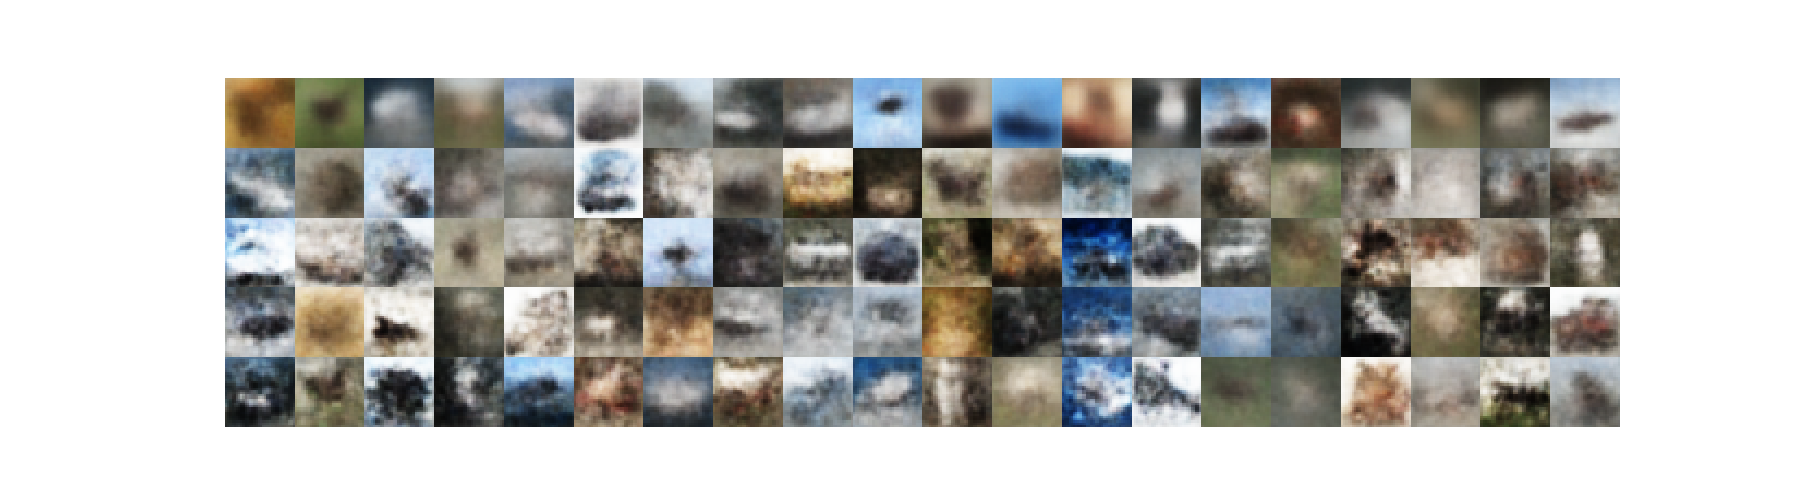
\includegraphics[width=\linewidth]{VAE_CIFAR_0_10_256.png}
    \caption{\small Results on latent size 10.} \label{fig:a}
    \end{subfigure}\hspace*{\fill}
    \begin{subfigure}{0.495\textwidth}
    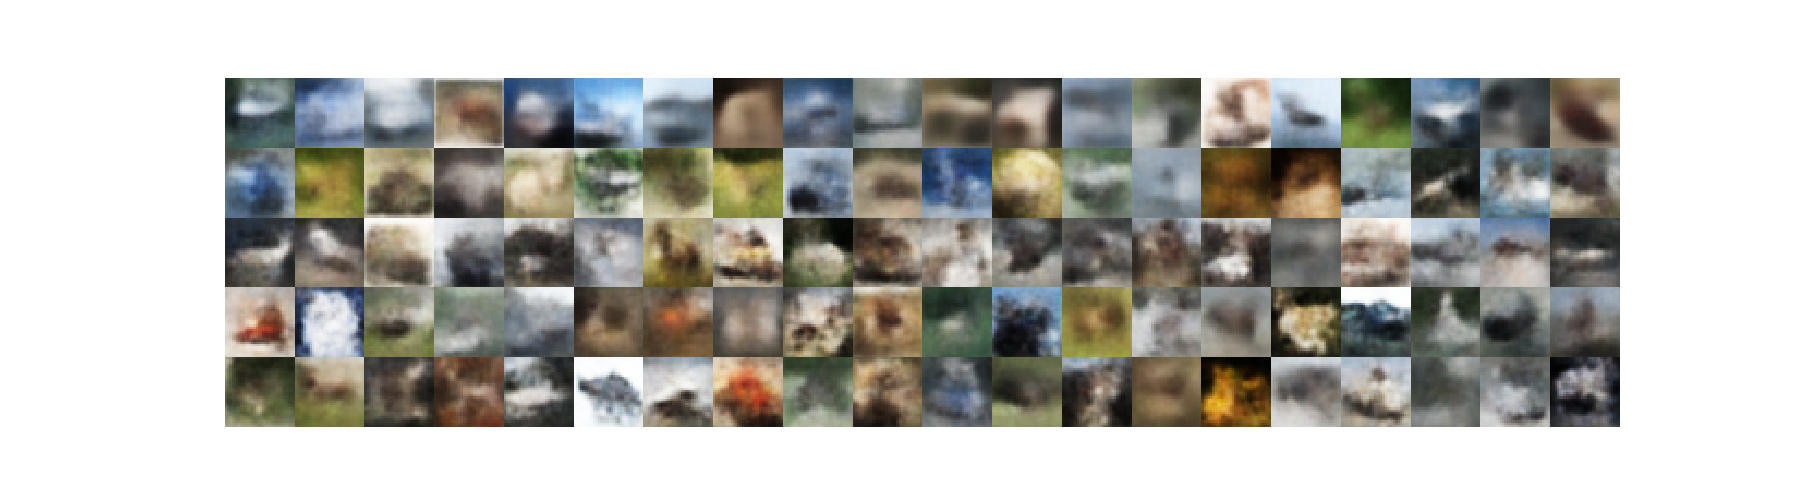
\includegraphics[width=\linewidth]{VAE_CIFAR_0_20_256.png}
    \caption{\small Results on latent size 20.} \label{fig:b}
    \end{subfigure}
    
    \medskip
    \begin{subfigure}{0.495\textwidth}
    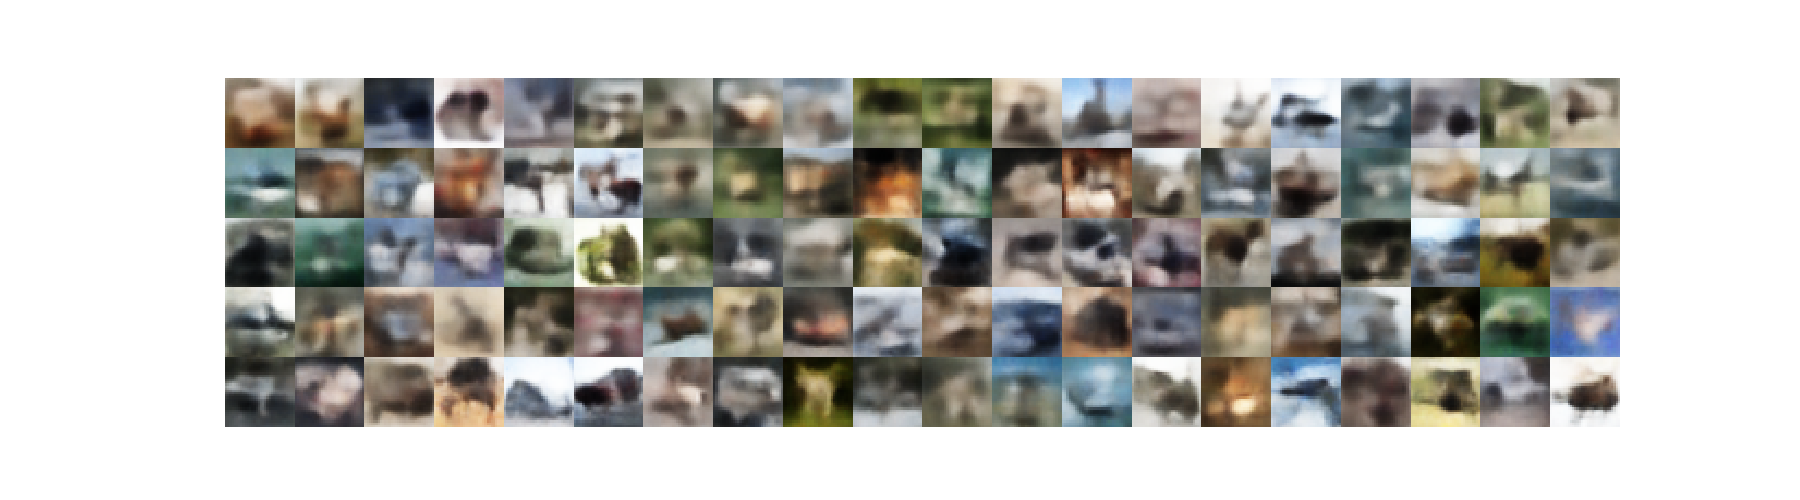
\includegraphics[width=\linewidth]{VAE_CIFAR_0_50_256.png}
    \caption{\small Results on latent size 50.} \label{fig:c}
    \end{subfigure}\hspace*{\fill}
    \begin{subfigure}{0.495\textwidth}
    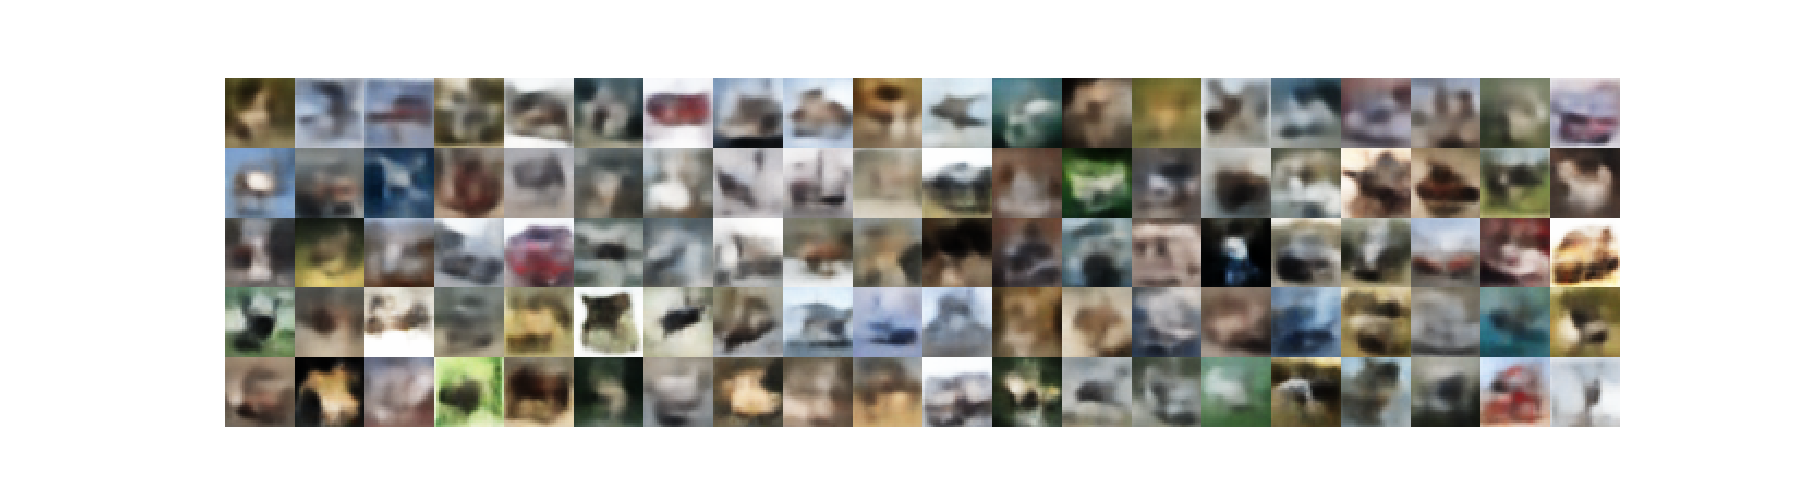
\includegraphics[width=\linewidth]{VAE_CIFAR_0_100_256.png}
    \caption{\small Results on latent size 100.} \label{fig:d}
    \end{subfigure}
    
    \hspace*{\fill}
    \caption{Influence of the latent size on $4$ models, with performance increasing row by row} \label{fig:CIFAR_VAE_latent}
\end{figure}

% To compare the influence of latent size, we fixed the number of hidden layers is $3$, and then compare latent size 10,20,50,100 and 200.

% Latent size 20 gets the better result than others. So, too small or too large latent size will reduce the performance of VAE.

In order to compare the training effort of the VAE model on different latent space sizes,
\begin{figure}[h]
    \centering
    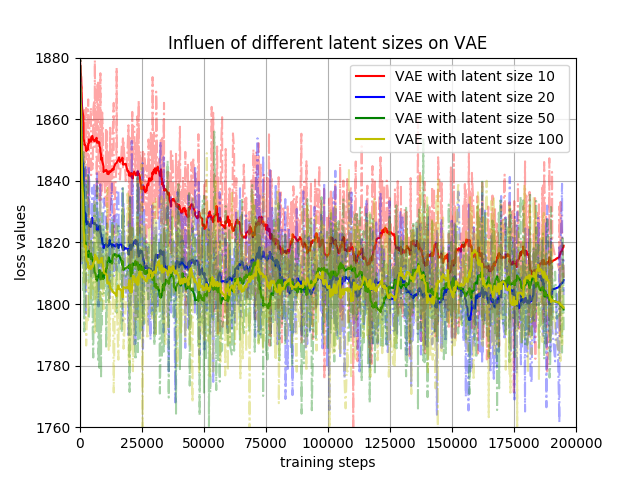
\includegraphics[width=.5\linewidth]{VAE_CIFAR_latents.png}
    \caption{\small Different latent size.}
    \label{fig:vae_latent_CIFAR}
\end{figure}

a plot of generator loss function value is created and plotted as Figure ~\ref{fig:vae_latent_CIFAR}


\begin{itemize}
    \item Compared to the VAE model on MNIST dataset, the training process of the VAE on the CIFAR dataset has the similar characters. This is because there exists only one loss function and both encoder and decoder are trained based on the gradient of that, which means the loss can be general smoother than GAN or WGAN.
    \item The loss value of VAE with latent size 100 and 50 are the lowest two finally in the plot. VAE needs more information to generate images in CIFAR10 datasets because images in this datasets are complex.
    \item The loss value of VAE with latent size 10 is the highest from start to end, which means CIFAR10 images is hard to generalize when given small latent size.
\end{itemize}

\subsubsection{Number of Hidden Layers}

First of all, let us take a look at the good quality results, which are shown as Figure ~\ref{fig:CIFAR_VAE_hidden_results} 

\begin{figure}[h]
    \centering
    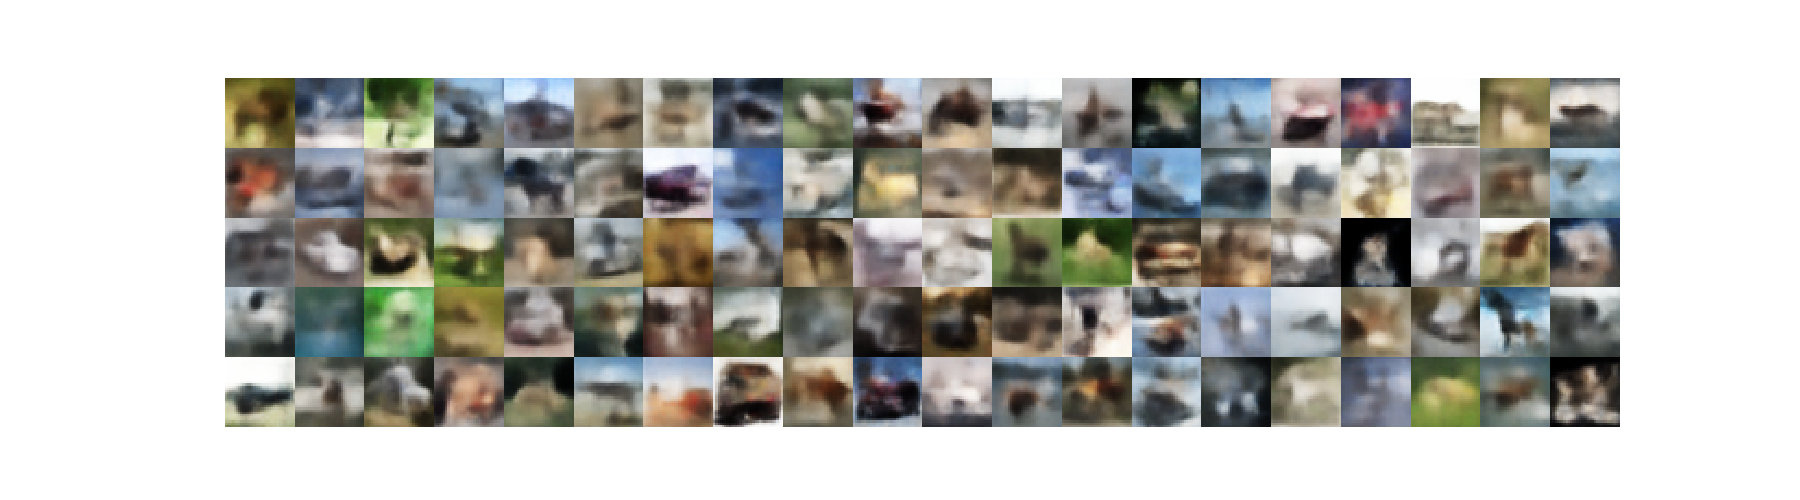
\includegraphics[width=.8\linewidth]{VAE_CIFAR_0_100_256results.png}
    \caption{\small A random sample with final results.}
    \label{fig:CIFAR_VAE_hidden_results}
\end{figure}

And increasing quality results are shown as Figure ~\ref{fig:CIFAR_VAE_hidden}

\begin{figure}[h]
    \begin{subfigure}{0.49\textwidth}
    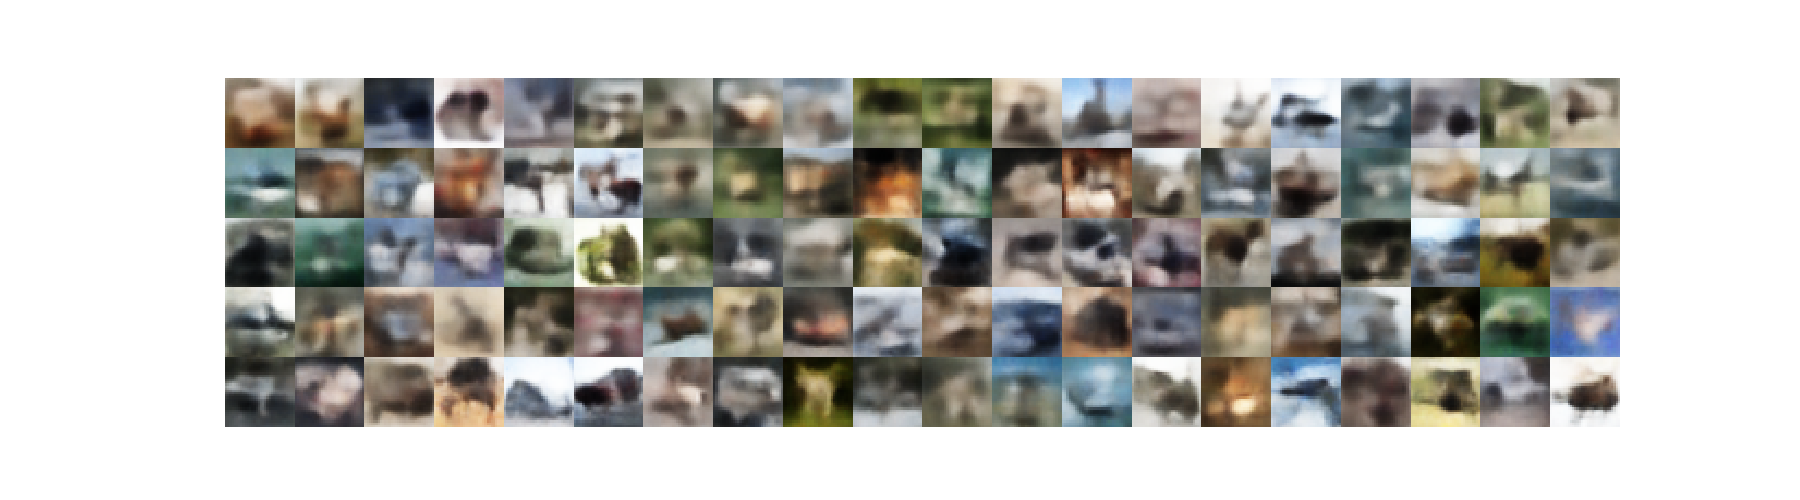
\includegraphics[width=\linewidth]{VAE_CIFAR_0_50_256.png}
    \caption{\small Results on 3 hidden layers} \label{fig:a}
    \end{subfigure}\hspace*{\fill}
    \begin{subfigure}{0.49\textwidth}
    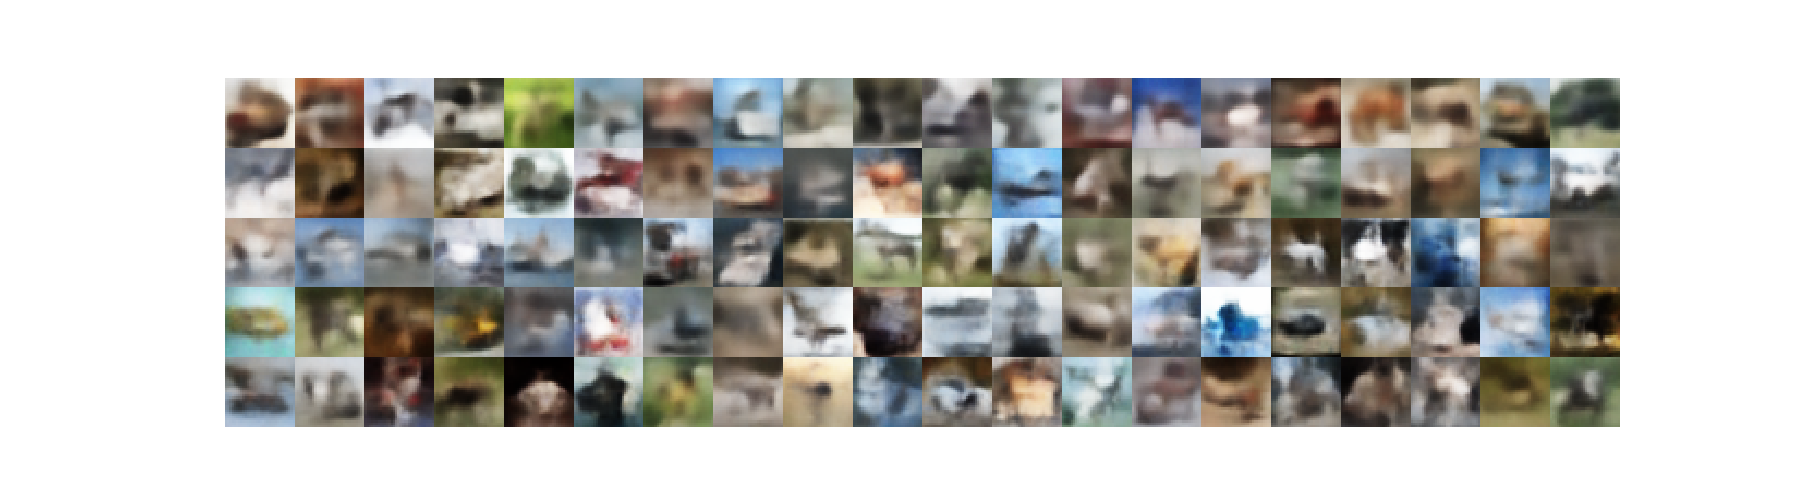
\includegraphics[width=\linewidth]{VAE_CIFAR_1_50_256.png}
    \caption{\small Results on 4 hidden layers} \label{fig:b}
    \end{subfigure}

    \medskip
    \begin{subfigure}{0.49\textwidth}
    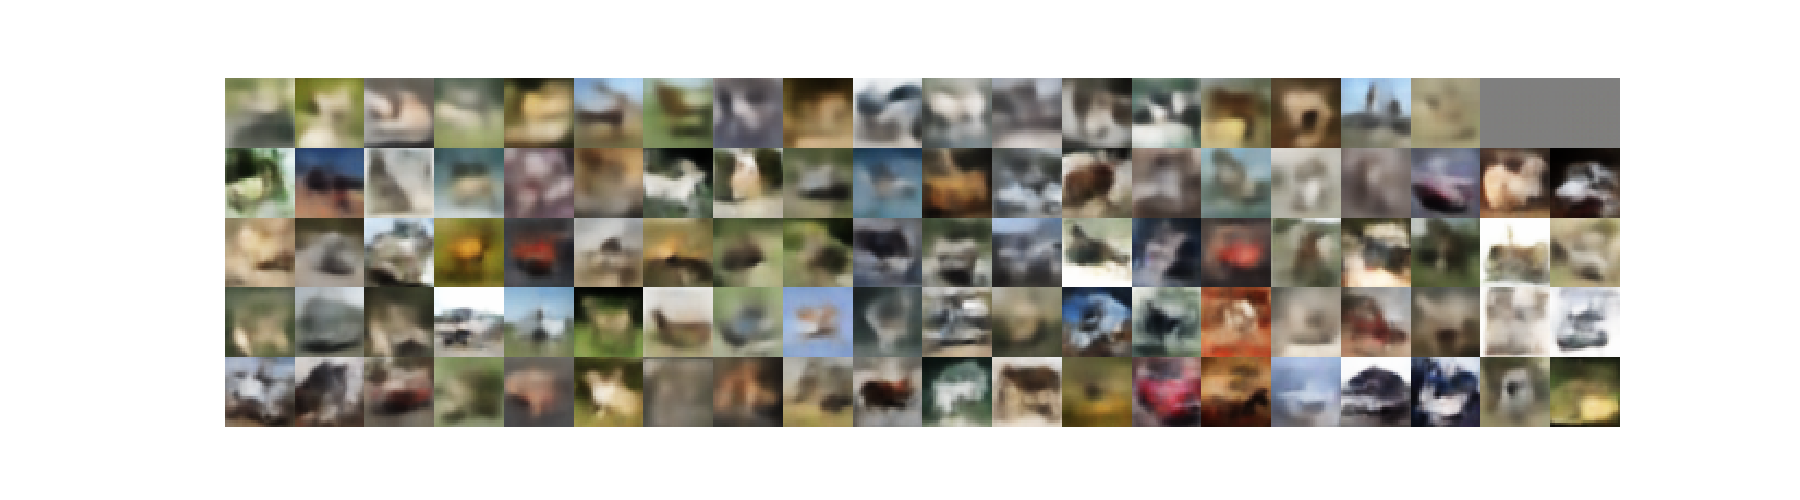
\includegraphics[width=\linewidth]{VAE_CIFAR_2_50_256.png}
    \caption{\small Results on 5 hidden layers} \label{fig:c}
    \end{subfigure}\hspace*{\fill}
    \caption{Influence of the number of hidden layers on $3$ models, with performance increasing row by row} \label{fig:CIFAR_VAE_hidden}
\end{figure}

In order to compare the training effort of the VAE model on different number of hidden layers, a plot of generator loss function value is created and plotted as Figure ~\ref{fig:vae_hidden_CIFAR}

\begin{figure}[h]
    \centering
    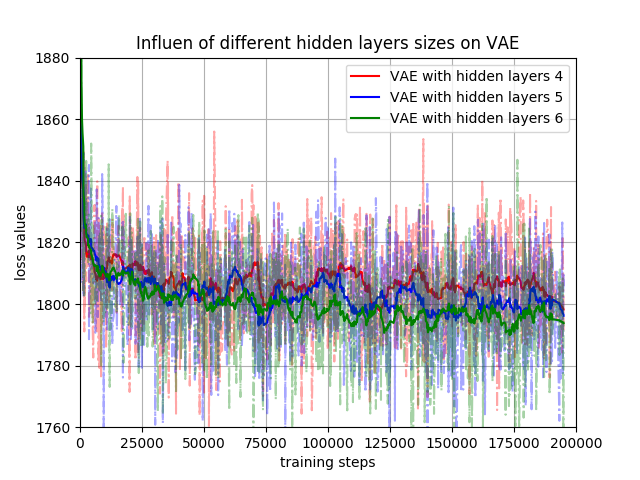
\includegraphics[width=.5\linewidth]{VAE_CIFAR_hidden.png}
    \caption{\small Different number of hidden layers.}
    \label{fig:vae_hidden_CIFAR}
\end{figure}

A brief conclusion is drawn as follow,
\begin{itemize}
    \item The loss value of VAE with 5 hidden layers is the lowest and this model can generate better images with more complex structure. This is possibly because images of CIFAR10 is so complex that VAE model needs more complex structure to learn it.
    \item Although the performances of the model with different complexities show a slight difference which has been observed and concluded above, One can, in general, say that the influence of the size of hidden layers cannot alter the performance of the model that much.
\end{itemize}


\subsection{GAN}

\subsubsection{Latent Size}

First of all, let us take a look at the good quality results, which are shown as Figure ~\ref{fig:CIFAR_GAN_latent_results} 

\begin{figure}[h]
    \centering
    \includegraphics[width=.8\linewidth]{GAN_CIFAR_0_10_256.png}
    \caption{\small A random sample with final results.}
    \label{fig:CIFAR_GAN_latent_results}
\end{figure}

And increasing quality results are shown as Figure ~\ref{fig:CIFAR_GAN_latent}

\begin{figure}[h]
    \begin{subfigure}{0.495\textwidth}
    \includegraphics[width=\linewidth]{GAN_CIFAR_0_10_256.png}
    \caption{\small Results on latent size 10.} \label{fig:a}
    \end{subfigure}\hspace*{\fill}
    \begin{subfigure}{0.495\textwidth}
    \includegraphics[width=\linewidth]{GAN_CIFAR_0_20_256.png}
    \caption{\small Results on latent size 20.} \label{fig:b}
    \end{subfigure}
    
    \medskip
    \begin{subfigure}{0.495\textwidth}
    \includegraphics[width=\linewidth]{GAN_CIFAR_0_50_256.png}
    \caption{\small Results on latent size 50.} \label{fig:c}
    \end{subfigure}\hspace*{\fill}
    \begin{subfigure}{0.495\textwidth}
    \includegraphics[width=\linewidth]{GAN_CIFAR_0_100_256.png}
    \caption{\small Results on latent size 100.} \label{fig:d}
    \end{subfigure}
    \caption{Influence of the latent size on $5$ models, with performance increasing row by row} \label{fig:CIFAR_GAN_latent}
\end{figure}

Apparently, the results are way shaper than those of VAE. This means, with certain training skills, GAN could get better prediction results than VAE. That is one possible reason why GAN is so welcomed all over the world.

In order to compare the training effort of the GAN model on different latent space sizes, a plot of generator loss function value is created and plotted as Figure ~\ref{fig:gen_latent_CIFAR}
\begin{figure}[h]
    \centering
    \includegraphics[width=.5\linewidth]{GAN_CIFAR_latents.png}
    \caption{\small Different latent size.}
    \label{fig:gen_latent_CIFAR}
\end{figure}

A brief conclusion is drawn as follow,
\begin{itemize}
    \item Generally speaking, the results follow agree on the knowledge we learnt from the class. The loss value goes up and the convergence speed slows down, which means the model is learning well on the dataset.
    \item One can say that the influence of different latent sizes on GAN can be neglected, since all the performances of these models show a lot similarities.
    \item In CIFAR10 datasets, we need more hidden layers to train these complex images. The best performances is reached when the number of hidden layers hits $4$, although only slight differnece could be captured.
    \item GAN with latent size 100 can generate well than other latent size models. This is possibly because CIFAR10 so complex that it needs more latent size to learn.
\end{itemize}

\subsubsection{Number of Hidden Layers}

First of all, let us take a look at the good quality results, which are shown as Figure ~\ref{fig:CIFAR_GAN_hidden_results} 
\begin{figure}[h]
    \centering
    \includegraphics[width=.8\linewidth]{GAN_CIFAR_0_50_256.png}
    \caption{\small A random sample with final results.}
    \label{fig:CIFAR_GAN_hidden_results}
\end{figure}

And increasing quality results are shown as Figure ~\ref{fig:CIFAR_GAN_hidden}
\begin{figure}[h]
    \begin{subfigure}{0.49\textwidth}
    \includegraphics[width=\linewidth]{GAN_CIFAR_0_50_256.png}
    \caption{\small Results on 3 hidden layers} \label{fig:a}
    \end{subfigure}\hspace*{\fill}
    \begin{subfigure}{0.49\textwidth}
    \includegraphics[width=\linewidth]{GAN_CIFAR_1_50_256.png}
    \caption{\small Results on 4 hidden layers} \label{fig:b}
    \end{subfigure}

    \medskip
    \begin{subfigure}{0.49\textwidth}
    \includegraphics[width=\linewidth]{GAN_CIFAR_2_50_256.png}
    \caption{\small Results on 5 hidden layers} \label{fig:c}
    \end{subfigure}\hspace*{\fill}
    \caption{Influence of the number of hidden layers on $3$ models, with performance increasing row by row} \label{fig:CIFAR_GAN_hidden}
\end{figure}

Same as before, the generated images are quite shape. Given more time training on it, we think the result could get better.

In order to compare the training effort of the GAN model on different number of hidden layers, a plot of generator loss function value is created and plotted as Figure ~\ref{fig:gen_hidden_CIFAR}
\begin{figure}[h]
    \centering
    \includegraphics[width=.5\linewidth]{GAN_CIFAR_hidden.png}
    \caption{\small Different number of hidden layers.}
    \label{fig:gen_hidden_CIFAR}
\end{figure}



A brief conclusion is drawn as follow,
\begin{itemize}
    \item GAN with 5 hidden layers gets the best result and this means larger and smaller number of hidden layers will reduce the performance.
    \item The generator loss value is still increasing when we stop iterations.Training GAN in CIFAR10 datasets needs more epochs, this shows that GAN is very difficult to train.
    \item Another thing we have to mention about the GAN is, the loss value goes extremely wild at the training process goes. This also meets the knowledge we have learnt in the class, which is it begins fluctuating at the beginning, then the magnitude of the oscillation becomes smaller and smaller. And finally, when the loss gets stable, the output results will become significantly promising.
\end{itemize}

\subsection{WGAN}

\subsubsection{Latent Size}

First of all, let us take a look at the good quality results, which are shown as Figure ~\ref{fig:CIFAR_WGAN_latent_results} 
\begin{figure}[h]
    \centering
    \includegraphics[width=.8\linewidth]{WGAN_CIFAR_0_50_256.png}
    \caption{\small A random sample with final results.}
    \label{fig:CIFAR_WGAN_latent_results}
\end{figure}

And increasing quality results are shown as Figure ~\ref{fig:CIFAR_WGAN_latent}

\begin{figure}[h]
    \begin{subfigure}{0.495\textwidth}
    \includegraphics[width=\linewidth]{WGAN_CIFAR_0_10_256.png}
    \caption{\small Results on latent size 10.} \label{fig:a}
    \end{subfigure}\hspace*{\fill}
    \begin{subfigure}{0.495\textwidth}
    \includegraphics[width=\linewidth]{WGAN_CIFAR_0_20_256.png}
    \caption{\small Results on latent size 20.} \label{fig:b}
    \end{subfigure}
    
    \medskip
    \begin{subfigure}{0.495\textwidth}
    \includegraphics[width=\linewidth]{WGAN_CIFAR_0_50_256.png}
    \caption{\small Results on latent size 50.} \label{fig:c}
    \end{subfigure}\hspace*{\fill}
    \begin{subfigure}{0.495\textwidth}
    \includegraphics[width=\linewidth]{WGAN_CIFAR_0_100_256.png}
    \caption{\small Results on latent size 100.} \label{fig:d}
    \end{subfigure}

    \caption{Influence of the latent size on $5$ models, with performance increasing row by row} \label{fig:CIFAR_WGAN_latent}
\end{figure}

Obviously, the quality of generated images of WGAN is worse than that of GAN. This does not necessarily mean that WGAN is no better than GAN. One possible reason is that since the WGAN requires weights clipping, it is naturally harder to train. If given enough time, I honestly think the performance of WGAN would be better than GAN.

In order to compare the training effort of the WGAN model on different latent space sizes, a plot of generator loss function value is created and plotted as Figure ~\ref{fig:wgen_latent_CIFAR}
\begin{figure}[h]
    \centering
    \includegraphics[width=.5\linewidth]{WGAN_CIFAR_latents.png}
    \caption{\small Different latent size.}
    \label{fig:wgen_latent_CIFAR}
\end{figure}

A brief conclusion is drawn as follow,
\begin{itemize}
    \item WGAN is typically hard to train. As one can observe, although the training step goes already over $800$, the loss still fluctuates a lot.
    \item WGAN can not generate images well in small latent size. In this plot, the WGAN with latent size 10 learnt extremely bad than other latent sizes. This is possibly because WGAN and other kind of GANs need more information to generate complex images.
    \item The reason why WGAN with latent size $10$ shows un-resonable results is probably that the latent size is too small and it requires WGAN takes much more time to start converge.
\end{itemize}

\subsubsection{Number of Hidden Layers}

First of all, let us take a look at the good quality results, which are shown as Figure ~\ref{fig:CIFAR_WGAN_hidden_results} 
\begin{figure}[h]
    \centering
    \includegraphics[width=.8\linewidth]{WGAN_CIFAR_0_50_256.png}
    \caption{\small A random sample with final results.}
    \label{fig:CIFAR_WGAN_hidden_results}
\end{figure}

And increasing quality results are shown as Figure ~\ref{fig:CIFAR_WGAN_hidden}

\begin{figure}[h]
    \begin{subfigure}{0.495\textwidth}
    \includegraphics[width=\linewidth]{WGAN_CIFAR_0_50_256.png}
    \caption{\small Results on 3 hidden layers} \label{fig:a}
    \end{subfigure}\hspace*{\fill}
    \begin{subfigure}{0.495\textwidth}
    \includegraphics[width=\linewidth]{WGAN_CIFAR_1_50_256.png}
    \caption{\small Results on 4 hidden layers} \label{fig:b}
    \end{subfigure}

    \medskip
    \begin{subfigure}{0.495\textwidth}
    \includegraphics[width=\linewidth]{WGAN_CIFAR_2_50_256.png}
    \caption{\small Results on 5 hidden layers} \label{fig:c}
    \end{subfigure}\hspace*{\fill}
    \caption{Influence of the number of hidden layers on $3$ models, with performance increasing row by row} \label{fig:CIFAR_WGAN_hidden}
\end{figure}

In order to compare the training effort of the WGAN model on different number of hidden layers, a plot of generator loss function value is created and plotted as Figure ~\ref{fig:wgen_hidden_CIFAR}

\begin{figure}[h]
    \centering
    \includegraphics[width=.5\linewidth]{WGAN_CIFAR_hidden.png}
    \caption{\small Different number of hidden layers.}
    \label{fig:wgen_hidden_CIFAR}
\end{figure}


A brief conclusion is drawn as follow,
\begin{itemize}
    \item WGAN with more hidden layers first learnt bad and then gradually learnt better and better. Finally, WGAN with 6 hidden layers gets the best results,and this shows that the complex model need to be applied to train complex dataset images.
    \item Since the hidden layer size $4$ is probably still not deep enough for the model to learn on such dataset, the loss value basically keeps a certain level during the whole training process, though one can still spot it decreases slightly.
\end{itemize}


\section{Other comments about training these models}

Some experience of building up hidden layers structure and tuning hyper-parameters:

\begin{itemize}
    \item Using LeakyRelu as the activation function of each hidden layer can improve the performance better.
    \item Adding Batch Normalization after each hidden layers rather than dropout, this is because dropout in generator will lose information, which leads to GAN and WGAN harder to train.
    \item Larger de-convolutional kernel size must be applied in generator when training higher quality images. In this assignment, the image quality of CIFAR10 is higher than MNIST. This is because high quality image features need to be extracted with more information.
    \item Only add one dropout layer after the flatten layer in discriminator, which can reduce over-fitting.
    \item Note: without these experience, the models can be trained well in MNIST datasets because the images in MNIST datasets are simple, meaning hands-writing images are learned by models easily. In CIFAR10 datasets, because images are more complex, models can not "tolerate" these problems without fine-tuning.
    \item Weight clipping range value is a key hyper-parameter to influence the model performance in WGAN, in this assignment, we used 0.01 as the clipping value, which is an experience value online. After we tuning this hyper-parameter, we found this experience value is the best we can find aimed to this assignment.
\end{itemize}

\end{document}